\documentclass[12pt,a4paper,oneside]{report}

\usepackage[utf8]{inputenc}
\usepackage[T1]{fontenc}
\usepackage{lmodern}
\usepackage[left=3.0cm, right=2.2cm, top=2.3cm, bottom=2.3cm]{geometry}
\usepackage{graphicx}
\usepackage{amsmath, amsfonts, amssymb}
\usepackage{fancyhdr}
\usepackage{titlesec}
\usepackage[table,xcdraw]{xcolor}
\usepackage[colorlinks=true, linkcolor=blue!70!black, urlcolor=blue!70!black, citecolor=blue!70!black]{hyperref}
\usepackage{booktabs}
\usepackage{longtable}
\usepackage{array}
\usepackage{caption}
\usepackage{subcaption}
\usepackage{tcolorbox}
\usepackage{listings}
\usepackage{setspace}
\usepackage{enumitem}
\usepackage{tikz}
\usetikzlibrary{shapes.geometric, arrows, positioning, fit, calc, shadows}

% Float & whitespace optimizations to fully utilize A4 format
\setlength{\headheight}{15pt}
\setlength{\headsep}{14pt}
\renewcommand{\topfraction}{0.90}
\renewcommand{\bottomfraction}{0.85}
\renewcommand{\textfraction}{0.10}
\renewcommand{\floatpagefraction}{0.80}
\captionsetup{font=small,labelfont={bf,color=gtublue},margin=6pt}
\captionsetup[sub]{font=footnotesize,labelfont={bf,color=black!85}}

\definecolor{gtublue}{RGB}{0, 51, 102}
\definecolor{gtured}{RGB}{204, 0, 0}
\definecolor{codebg}{RGB}{245, 245, 245}
\definecolor{codegray}{rgb}{0.5,0.5,0.5}
\definecolor{codepurple}{rgb}{0.58,0,0.82}
\definecolor{backcolour}{rgb}{0.95,0.95,0.92}
\definecolor{defgreen}{RGB}{22, 122, 60}
\definecolor{defred}{RGB}{180, 40, 40}

\tcbuselibrary{skins,breakable}

\newtcolorbox{defensebox}[1]{
    colback=blue!5!white, colframe=gtublue, fonttitle=\bfseries,
    title=#1, boxrule=1pt, arc=4pt, breakable
}
\newtcolorbox{codebox}[1]{
    colback=backcolour, colframe=black!70, fonttitle=\bfseries,
    title=#1, boxrule=1pt, arc=2pt, breakable
}
\newtcolorbox{resultbox}[1]{
    colback=green!4!white, colframe=defgreen, fonttitle=\bfseries,
    title=#1, boxrule=1pt, arc=4pt, breakable
}
\newtcolorbox{negativebox}[1]{
    colback=red!4!white, colframe=defred, fonttitle=\bfseries,
    title=#1, boxrule=1pt, arc=4pt, breakable
}

\lstdefinestyle{mystyle}{
    backgroundcolor=\color{backcolour}, commentstyle=\color{green!50!black},
    keywordstyle=\color{magenta}, numberstyle=\tiny\color{codegray},
    stringstyle=\color{codepurple}, basicstyle=\ttfamily\footnotesize,
    breakatwhitespace=false, breaklines=true, captionpos=b, keepspaces=true,
    numbers=left, numbersep=5pt, showspaces=false, showstringspaces=false,
    showtabs=false, tabsize=2
}
\lstset{style=mystyle}

\pagestyle{fancy}
\fancyhf{}
\fancyhead[L]{\textcolor{gtublue}{\textbf{Pramaan: Minor Project DI05000341}}}
\fancyhead[R]{\nouppercase{\leftmark}}
\fancyfoot[C]{\thepage}
\renewcommand{\headrulewidth}{0.6pt}
\renewcommand{\footrulewidth}{0.6pt}

\titleformat{\chapter}[display]
  {\normalfont\Huge\bfseries\color{gtublue}}{\chaptertitlename\ \thechapter}{10pt}{\Huge}[\vspace{1ex}\titlerule]
\titlespacing*{\chapter}{0pt}{-10pt}{20pt}
\titleformat{\section}{\normalfont\Large\bfseries\color{black!80}}{\thesection}{1em}{}
\titlespacing*{\section}{0pt}{12pt plus 3pt minus 2pt}{5pt plus 1pt minus 1pt}
\titleformat{\subsection}{\normalfont\large\bfseries\color{black!70}}{\thesubsection}{1em}{}
\titlespacing*{\subsection}{0pt}{10pt plus 2pt minus 1pt}{4pt plus 1pt minus 1pt}

\setstretch{1.18}
\renewcommand{\arraystretch}{1.20}
\setlength{\parskip}{3pt plus 1pt minus 1pt}

\newcommand{\rupee}{Rs.\ }
% Per-member printed copies (identical content; only the deposit line differs)
\newcommand{\memberLead}{Aayush Avinash Bankar}
\newcommand{\memberEnrol}{246230316006}
\newcommand{\otherName}{Meet Jayeshbhai Patel}
\newcommand{\otherEnrol}{246230316133}
\newcommand{\memberRole}{Team Leader}
\newcommand{\otherRole}{Team Member}
\newcommand{\copyNo}{1}
\newcommand{\runid}[1]{\texttt{#1}}

\begin{document}

% ================= TITLE PAGE =================
\begin{titlepage}
    \begin{center}
        \vspace*{0.1cm}
        \LARGE
        \textbf{\textcolor{gtured}{GUJARAT TECHNOLOGICAL UNIVERSITY}}

        \vspace{0.4cm}
        \large
        \textbf{Programme: Diploma Engineering \quad Level: Diploma \quad Semester: $5^{th}$} \\
        \textbf{Subject Code: DI05000341 \quad Subject Name: Minor Project}

        \vspace{0.4cm}
        \rule{\textwidth}{1pt}
        \vspace{0.25cm}

        \Huge
        \textbf{\textcolor{gtublue}{Pramaan}} \\
        \vspace{0.1cm}
        \normalsize
        \textit{(Sanskrit pram\={a}na --- proof, evidence)} \\
        \vspace{0.15cm}
        \Large
        \textbf{\textit{Prove your edge before you deploy a rupee.}} \\
        \vspace{0.15cm}
        \large
        An event-driven backtesting engine and overfitting diagnostic platform \\
        for Indian equities

        \vspace{0.25cm}
        \rule{\textwidth}{1pt}
        \vspace{0.5cm}

        \textbf{Submitted by} \\[0.2cm]
        {\Large \textbf{\memberLead} \quad \memberRole} \\
        \textbf{Enrolment: \memberEnrol} \\[0.1cm]
        {\large \textbf{\otherName} \quad \otherRole} \\
        \textbf{Enrolment: \otherEnrol}

        \vspace{0.25cm}
        \normalsize\itshape
        Submitted in partial fulfilment of the requirements for the Diploma in Engineering

        \vspace{0.3cm}
        \normalsize
        \texttt{Team copy \copyNo\ of 2 --- deposited by \memberLead}

        \vfill
        \large
        \textbf{Academic Year 2026--27} \\
        \normalsize
        Gujarat, India
    \end{center}
\end{titlepage}

% ================= CERTIFICATE =================
\chapter*{Certificate}
\addcontentsline{toc}{chapter}{Certificate}
\thispagestyle{plain}

\vspace{1cm}
\begin{center}
    \textbf{\large CERTIFICATE}
\end{center}
\vspace{0.8cm}

This is to certify that the minor project entitled

\begin{center}
    \textbf{\large ``Pramaan: An Event-Driven Backtesting Engine and Overfitting}\\
    \textbf{\large Diagnostic Platform for Indian Equities''}
\end{center}

is a record of the bonafide work carried out and submitted by

\begin{center}
    \textbf{Aayush Avinash Bankar} (246230316006) \\
    \textbf{Meet Jayeshbhai Patel} (246230316133)
\end{center}

in partial fulfilment of the requirements for the award of the Diploma in Engineering
(Semester 5, Subject Code DI05000341), and that the work has been carried out under
supervision and guidance in accordance with the curriculum of Gujarat Technological
University.

The results embodied in this report have not been submitted to any other University
or Institute for the award of any degree or diploma.

\vspace{2.5cm}

\begin{flushleft}
\begin{tabular}{@{}p{7cm}p{6cm}@{}}
\rule{6cm}{0.4pt} & \rule{6cm}{0.4pt} \\
\textbf{Prof. / Head of Department} & \textbf{Project Guide} \\
Computer Engineering & Computer Engineering \\
Govt. Polytechnic Gandhinagar & Govt. Polytechnic Gandhinagar \\
\end{tabular}

\vspace{2cm}

\begin{tabular}{@{}p{7cm}p{6cm}@{}}
\rule{6cm}{0.4pt} & \rule{6cm}{0.4pt} \\
\textbf{External Examiner} & \textbf{Date} \\
 & \\
\end{tabular}
\end{flushleft}

% ================= DECLARATION =================
\chapter*{Declaration}
\addcontentsline{toc}{chapter}{Declaration}
\thispagestyle{plain}

\vspace{1cm}

We, the undersigned, hereby declare that the project report entitled
``\textbf{Pramaan: An Event-Driven Backtesting Engine and Overfitting Diagnostic
Platform for Indian Equities}'' is the result of our own work. All sources of
information and materials that have been used in this project are duly
acknowledged.

We further declare that:

\begin{enumerate}[leftmargin=1.5cm]
    \item The backtesting engine, cost model, and statistical diagnostics presented
    in this report were implemented by us from first principles in Python. No
    third-party backtesting library (Backtrader, Zipline, LEAN, VectorBT) was used
    as a substitute for the engine core.
    \item All numerical results reported were produced by executing our own engine
    over historical NSE data and are reproducible from the artifacts committed in
    this repository. No result was hand-edited or fabricated.
    \item Where a claim is presented as a limitation or an unresolved question, it
    is identified as such in the text.
\end{enumerate}

\vspace{2cm}

\begin{flushleft}
\begin{tabular}{@{}p{7cm}p{6cm}@{}}
\rule{6cm}{0.4pt} & \rule{6cm}{0.4pt} \\
\textbf{Aayush Avinash Bankar} & \textbf{Meet Jayeshbhai Patel} \\
246230316006 & 246230316133 \\
Date: \underline{\hspace{3cm}} & Date: \underline{\hspace{3cm}} \\
\end{tabular}
\end{flushleft}

% ================= ACKNOWLEDGEMENT =================
\chapter*{Acknowledgement}
\addcontentsline{toc}{chapter}{Acknowledgement}
\thispagestyle{plain}

\vspace{0.8cm}

We would like to express our sincere gratitude to our project guide for the
continuous mentorship, technical criticism, and scholarly direction that shaped
this work, and to the Head of the Computer Engineering Department and the faculty
of Government Polytechnic Gandhinagar for providing the laboratory infrastructure
and academic environment necessary to carry out this project.

We thank the faculty whose lectures in data structures, algorithms, statistics,
and database management systems supplied the foundational techniques applied here,
in particular the treatment of time-series correlation, ordinary differential
equations used as an analogy for portfolio dynamics, and the principles of
deterministic system design.

We are grateful to the Securities and Exchange Board of India (SEBI) and the
National Stock Exchange of India (NSE) for publishing their rate schedules and
empirical retail-performance studies as open references; without those documents,
this project would have been a generic simulation with no relation to real Indian
market microstructure.

We acknowledge the open-source research community: Dr.\ Marcos López de Prado's
work on the Deflated Sharpe Ratio and Combinatorial Purged Cross-Validation, and
Almgren and Chriss's work on optimal execution and market impact, were the direct
theoretical foundations of the analytics module. We also acknowledge the
maintainers of NumPy, pandas, and SciPy, whose libraries formed the numerical
substrate of our implementation.

Finally, we thank our families and classmates who tested the dashboard, asked the
questions that exposed our look-ahead assumptions, and refused to accept vague
answers.

% ================= ABSTRACT =================
\chapter*{Abstract}
\addcontentsline{toc}{chapter}{Abstract}
\thispagestyle{plain}

\vspace{0.5cm}

Retail and discretionary trading strategies that appear profitable in a naive
historical backtest routinely fail in live markets. This report presents
\textbf{Pramaan}, an event-driven backtesting engine and overfitting diagnostic
platform built from first principles for Indian equity markets, which attacks
three specific causes of that failure: hidden statutory transaction costs,
hidden market impact on execution price, and hidden statistical overfitting.

The engine enforces a \emph{zero look-ahead} invariant by construction: a
strategy may only observe market data up to a given trading day's close, and any
order generated from that signal can only be filled at the following day's
opening price. A complete Indian statutory cost stack --- brokerage, securities
transaction tax (STT), stamp duty, NSE and SEBI turnover charges, and GST --- is
applied per fill, together with an Almgren--Chriss square-root market-impact
model calibrated against trailing volatility and average daily volume. Overfitting
is quantified using the Deflated Sharpe Ratio and Combinatorial Purged
Cross-Validation with embargo, the latter equipped with an autocorrelation test
that demonstrates leakage at block boundaries.

The system was evaluated on real National Stock Exchange daily data: ten large-cap
symbols, 1{,}480 trading bars each, spanning 2019-01-01 to 2024-12-30, with
thirty completed backtest configurations. The results are reported without
embellishment. Under realistic costs, \emph{no} active strategy among
SMA-crossover, RSI mean-reversion, and momentum exceeded a naive buy-and-hold
benchmark on a risk-adjusted basis; the best active configuration achieved a
Sharpe ratio of 0.685 against the benchmark's 0.746. Enabling the statutory cost
stack removed 48.2\% of the momentum strategy's Sharpe ratio and
\rupee{}12{,}995 of terminal equity on a \rupee{}1{,}00{,}000 starting capital.
Combinatorial Purged Cross-Validation reported a probability of backtest
overfitting of 64.29\% across the tested configurations.

These outcomes are consistent with the near-efficient market hypothesis for
large-cap Indian equities and are presented as the central finding of the
project. The engine, its validation statistics, and its regression test suite
(35 automated tests, all passing) are released under Apache License 2.0.

\textbf{Keywords:} backtesting, look-ahead bias, overfitting, Deflated Sharpe
Ratio, Combinatorial Purged Cross-Validation, Almgren--Chriss market impact,
Indian equity market microstructure, STT, NSE.

% ================= FRONT MATTER =================
\pagenumbering{roman}
\tableofcontents
\clearpage
\listoffigures
\clearpage
\listoftables
\clearpage
\pagenumbering{arabic}

% ================= CHAPTER 1 =================
\chapter{Literature Survey and Problem Identification}

\section{The Problem: Trading Strategies That Lie}

The motivating observation of this project is simple and empirically well
documented: \emph{a profitable backtest is not evidence of a profitable strategy}.
A strategy can be simulated, tuned, and evaluated over a decade of historical data
and still lose money from the day it is deployed. The reason is not a shortage of
computation; it is that standard backtesting pipelines systematically omit the
mechanisms through which a live trading strategy loses capital.

This project identifies and models three such mechanisms, which we refer to as
the \emph{three silent killers}.

\begin{itemize}[leftmargin=1cm]
    \item \textbf{Cost blindness.} A strategy that trades twenty times a year
    pays the full Indian statutory cost stack on every round trip. These are not
    negligible: securities transaction tax is levied on both the buy and sell
    legs, stamp duty on the buy leg, exchange and SEBI turnover charges on both,
    and GST applies to brokerage and turnover. A strategy with a 5\% gross annual
    return and meaningful turnover can easily be rendered net-negative.
    \item \textbf{Execution blindness.} Orders of a size comparable to average
    daily volume move the market. A simulator that fills every order at the
    closing price systematically overstates achievable returns, and the
    overstatement grows with position size --- precisely when the trader needs a
    more honest estimate.
    \item \textbf{Selection blindness.} A researcher who tests one hundred
    parameter combinations and reports the best one has not found an edge; they
    have found a local maximum of a sample path. Reported Sharpe ratios are then
    upward-biased by the multiple-comparison effect, and any conventional
    confidence interval computed on that selection is invalid.
\end{itemize}

\section{Indian Market Context}

The SEBI empirical studies of Indian retail performance provide a stark
motivation. A 2024 SEBI study of futures-and-options retail participation
reported that a large majority of individual traders incurred net losses, and a
parallel study of cash-market active trading reported a comparable majority
loss rate with aggregate individual losses on the order of \rupee{}1.81 lakh
crore. The standard explanations --- lack of funds, lack of information --- are
only part of the picture. A substantial and often ignored component is the
\emph{friction game}: converting a positive-sum equity exposure into a
negative-sum trading vehicle by paying statutory costs and market impact on
every round trip, while believing a backtest that ignored them.

This project therefore deliberately restricts itself to \textbf{NSE cash
equities} and to \textbf{daily bars}. That restriction is not a limitation of
capability; it is the boundary within which the cost model and validation
statistics can be modelled with defensible accuracy.

\section{Research Questions and Hypotheses}

The project is organised around four research questions.

\begin{center}
\begin{tabular}{@{}p{0.7cm}p{12cm}@{}}
\textbf{RQ1} & Does enforcing a zero look-ahead, next-open execution rule
materially change backtest outcomes relative to a naive close-price fill? \\
\textbf{RQ2} & Does applying the full Indian statutory cost stack materially
degrade reported performance, and by how much, per strategy? \\
\textbf{RQ3} & Do classic technical strategies on large-cap NSE equities exhibit
positive risk-adjusted alpha relative to a naive buy-and-hold benchmark after
realistic costs? \\
\textbf{RQ4} & Is the probability of backtest overfitting across a small
parameter family high enough that conventional in-sample selection is
misleading? \\
\end{tabular}
\end{center}

The corresponding null and alternative hypotheses for the core claim (RQ3) were:

\begin{defensebox}{Hypotheses}
$H_0$: after the full statutory cost stack, the risk-adjusted performance of each
tested technical strategy is no greater than that of a naive buy-and-hold
benchmark over the same universe and period.

$H_1$: at least one tested technical strategy achieves a materially higher
risk-adjusted ratio than the benchmark after the full statutory cost stack.
\end{defensebox}

Section~\ref{ch:results} demonstrates that the data \textbf{do not} provide
grounds to reject $H_0$: all four active configurations underperformed the
benchmark. That is the project's central result, and it is reported as a
negative result in the strongest sense --- one that the engine was built to
detect.

\section{Objectives}

\begin{enumerate}[leftmargin=1cm]
    \item Implement an event-driven simulation engine whose execution model
    renders look-ahead bias structurally impossible rather than merely unlikely.
    \item Implement a statutory Indian cost model that computes each levy
    correctly, including side-dependence and rounding rules.
    \item Implement a market-impact model that scales with order size relative
    to traded volume.
    \item Implement overfitting diagnostics --- Deflated Sharpe Ratio and
    Combinatorial Purged Cross-Validation with embargo --- and validate their
    behaviour on synthetic processes whose ground truth is known.
    \item Evaluate classic strategies on real NSE data and report the outcome
    honestly, including any result that contradicts the premise of the work.
\end{enumerate}

\section{Scope and Limitations (stated up front)}

\begin{itemize}[leftmargin=1.5cm]
    \item Simulation and validation only. Pramaan does not connect to a broker,
    does not place orders, and does not execute trades.
    \item Daily bars. No intraday, tick, or minute-level data.
    \item NSE cash equities only. No options, futures, commodities, or crypto.
    \item Long-only positions. No short selling, margin, or leverage.
    \item Backtests assume full fill of market orders at the modelled price.
\end{itemize}

These boundaries are stated here rather than discovered later, because in this
project limitations are treated as part of the result. A viva panel is entitled
to know them before the demonstration begins.

\section{Survey of Existing Backtesting Tools}

A requirement of this project was to justify building an engine rather than
adopting one. The comparison below drove that decision. The decisive column for
an Indian equity study is not speed or feature count --- it is whether the tool
models the statutory cost stack and reports selection-bias diagnostics.

\begin{table}[h]
\centering
\caption[Backtesting Approaches Comparison]{Comparison of available backtesting approaches against this project's requirements.}
\label{tab:competitors}
\begin{tabular}{@{}p{3.1cm}p{2.1cm}p{2.0cm}p{2.0cm}p{3.2cm}@{}}
\toprule
\textbf{Tool} & \textbf{Exec.\ model} & \textbf{Indian costs} & \textbf{DSR / CPCV} & \textbf{Verdict for this project} \\
\midrule
Backtrader & Event-driven & No & No & Dormant upstream; no Indian levy model. \\
Zipline & Event-driven & No & No & Upstream project retired; unsuitable as a dependency. \\
LEAN / QuantConnect & Event-driven & No & Partial & Cloud-priced; built for institutional multi-asset use. \\
VectorBT & Vectorised & No & No & Vectorised fills cannot enforce a next-bar open boundary. \\
Backtesting.py & Vectorised & No & No & Tight licence; close-price fill assumption. \\
MetaTrader & Event-driven & No & No & FX/CFD oriented; broker-dependent data. \\
TradingView & Scripted & No & No & Pine scripts have no execution model of this kind. \\
\midrule
\textbf{Pramaan} & \textbf{Event-driven} & \textbf{Yes} & \textbf{Yes} & \textbf{Built to the requirements below.} \\
\bottomrule
\end{tabular}
\end{table}

Two observations from this survey were decisive. First, the vectorised tools are
faster precisely because they process the entire dataframe at once, which is
structurally incompatible with claiming that a signal cannot see the future.
Speed was therefore deliberately traded for correctness of the execution model.
Second, there is \emph{no} off-the-shelf tool that models the Indian statutory
cost stack, and none reports a Deflated Sharpe Ratio with purged
cross-validation. Building was justified not by preference but by the absence of
the required capability.

It is worth recording the counter-argument honestly: adopting a mature library
would have saved roughly 1{,}000 lines of implementation and would have brought
an established user community. It would also have produced a project in which the
essential mechanism --- the execution boundary and the cost model --- was a
library's behaviour rather than this team's understanding of it. The build was
chosen because the point of the minor project is the mechanism, not the tool.

% ================= CHAPTER 2 =================
\chapter{System Specification and Design}

\section{Software Requirements}

\subsection{Functional Requirements}

\begin{center}
\begin{longtable}{@{}p{1.4cm}p{11.5cm}@{}}
\toprule
\textbf{ID} & \textbf{Requirement} \\
\midrule
\endfirsthead
FR-1 & System shall fetch and retain historical OHLCV data for a defined set of NSE equities. \\
FR-2 & System shall clean data by dropping incomplete bars, de-duplicating dates, and sorting chronologically; forward-filling is prohibited. \\
FR-3 & System shall implement a minimum of three trading strategies (SMA crossover, RSI mean-reversion, momentum) behind a common interface. \\
FR-4 & System shall generate buy/sell signals per strategy per trading day. \\
FR-5 & System shall simulate order execution at the next day's open, never at the signal bar's close. \\
FR-6 & System shall apply the full Indian statutory cost stack and a size-aware market-impact model to every fill. \\
FR-7 & System shall support position sizing as a fixed fraction of total portfolio equity. \\
FR-8 & System shall compute total return, CAGR, Sharpe, Sortino, Calmar, and maximum drawdown. \\
FR-9 & System shall compute the Deflated Sharpe Ratio for a stated number of trials. \\
FR-10 & System shall compute Combinatorial Purged Cross-Validation paths and the Probability of Backtest Overfitting. \\
FR-11 & System shall toggle the cost stack on and off to quantify its effect. \\
FR-12 & System shall log every run --- strategy, parameters, universe, date range, cost setting, metrics --- with a deterministic run identifier. \\
FR-13 & System shall expose a reproducible artifact set: experiment log, decay table, provenance record. \\
FR-14 & System shall provide a naive buy-and-hold benchmark as a control condition. \\
FR-15 & System shall expose the engine through a RESTful HTTP API and a command-line entry point. \\
\bottomrule
\end{longtable}
\end{center}

\subsection{Non-Functional Requirements}

\begin{center}
\begin{longtable}{@{}p{1.4cm}p{11.5cm}@{}}
\toprule
\textbf{ID} & \textbf{Requirement} \\
\midrule
\endfirsthead
NFR-1 & \textbf{Determinism.} Identical inputs must produce a byte-identical equity curve. Verified by test (\S\ref{sec:testing}). \\
NFR-2 & \textbf{Performance.} A ten-symbol, six-year daily backtest should complete within sixty seconds on commodity hardware. \\
NFR-3 & \textbf{Decoupling.} The engine, analytics, strategy, and data layers must be independently importable and testable without the UI. \\
NFR-4 & \textbf{Transparency.} Every reported metric must be traceable to a documented formula and a run artifact. \\
NFR-5 & \textbf{Zero-cost data.} The pipeline must operate on freely obtainable data. \\
NFR-6 & \textbf{Traceability.} Every claim about the system must have an associated verification record. \\
\bottomrule
\end{longtable}
\end{center}

\section{System Architecture}

The system is deliberately layered so that each layer can be tested in isolation.
Critically, the engine has \emph{no} dependency on the presentation layer: it runs
headlessly with no streaming or web framework present.

\begin{figure}[h]
\centering
\begin{tikzpicture}[
    node distance=1.6cm, auto,
    box/.style={rectangle, rounded corners, minimum width=12.5cm, minimum height=1.05cm,
                text centered, draw=black, fill=blue!8, font=\small},
    core/.style={rectangle, rounded corners, minimum width=12.5cm, minimum height=1.05cm,
                 text centered, draw=gtured, fill=red!8, font=\small, line width=1.2pt},
    lab/.style={font=\footnotesize\itshape}
]
    \node (ui)   [box, fill=blue!12] {\textbf{Presentation} \quad Next.js 15 Workstation $\cdot$ Streamlit fallback $\cdot$ CLI};
    \node (api)  [box] {\textbf{API (FR-15)} \quad FastAPI REST service $\cdot$ Pydantic validation $\cdot$ Cache/Replay provenance};
    \node (an)   [box] {\textbf{Analytics} \quad metrics $\cdot$ Deflated Sharpe $\cdot$ CPCV + embargo $\cdot$ grid search};
    \node (eng)  [core] {\textbf{Engine (the contribution)} \quad BacktestEngine $\cdot$ Portfolio $\cdot$ Position $\cdot$ IndianCostModel};
    \node (strat)[box] {\textbf{Strategy} \quad SMA $\cdot$ RSI $\cdot$ Momentum $\cdot$ BuyAndHold};
    \node (data) [box] {\textbf{Data} \quad fetch $\cdot$ clean $\cdot$ universe $\cdot$ Parquet cache};
    \draw [thick,->,>=stealth] (ui) -- (api);
    \draw [thick,->,>=stealth] (api) -- (an);
    \draw [thick,->,>=stealth] (an) -- (eng);
    \draw [thick,->,>=stealth] (strat) -- (eng);
    \draw [thick,->,>=stealth] (data) -- (eng);
    \node [lab, right=0.25cm of eng, xshift=-6.4cm, yshift=0.55cm] {\textcolor{gtured}{untouched, regression-tested}};
\end{tikzpicture}
\caption[Layered System Architecture]{Layered architecture. The engine is the academic contribution and is never rewritten.}
\label{fig:layers}
\end{figure}

\section{The Zero Look-Ahead Execution Model}

The central architectural decision of the project is the structure of the
simulation clock. A vectorised implementation computes all signals from the
complete dataframe in one operation, which makes it structurally impossible to
prevent a signal from reading a bar that had not yet traded. Pramaan therefore
uses an explicit event loop with a one-bar delay between decision and execution.

\begin{figure}[h]
\centering
\begin{tikzpicture}[
    node distance=1.4cm, auto,
    ss/.style={rectangle, rounded corners, minimum width=4.2cm, minimum height=1cm,
               text centered, draw=black, fill=blue!12, font=\small\bfseries},
    pr/.style={rectangle, minimum width=4.2cm, minimum height=1cm,
               text centered, draw=black, fill=gray!10, font=\small},
    ar/.style={thick,->,>=stealth}
]
    \node (dayT)  [ss, align=center] {Day $t$\\Market Close};
    \node (slice) [pr, below of=dayT] {Strategy sees data $\le t$ only};
    \node (sig)   [pr, below of=slice] {SignalEvent generated};
    \node (queue) [pr, below of=sig] {OrderEvent $\rightarrow$ \textsc{PendingOrders}};
    \node (dayT1) [ss, right of=queue, xshift=4.4cm, align=center] {Day $t+1$\\Market Open};
    \node (fill)  [pr, above of=dayT1] {Order filled at \textbf{Open}};
    \node (cost)  [pr, above of=fill] {Cost stack + Almgren--Chriss impact};
    \node (ledger)[pr, above of=cost] {FillEvent $\rightarrow$ Portfolio ledger};
    \draw [ar] (dayT) -- (slice);
    \draw [ar] (slice) -- (sig);
    \draw [ar] (sig) -- (queue);
    \draw [ar] (queue) -- (dayT1);
    \draw [ar] (dayT1) -- (fill);
    \draw [ar] (fill) -- (cost);
    \draw [ar] (cost) -- (ledger);
\end{tikzpicture}
\caption[One-Bar Zero-Lookahead Execution Boundary]{The one-bar execution boundary. A signal generated at bar $t$'s close cannot be filled before bar $t+1$'s open.}
\label{fig:timeline}
\end{figure}

\begin{codebox}{Next-open enforcement (\texttt{src/engine/backtest\_engine.py})}
\begin{lstlisting}[language=Python]
# 1. T+1 OPEN: execute orders queued at the previous close
self._execute_pending_orders(current_date)

# 2. T CLOSE: signals may only see bars up to and including today
sliced_data = {sym: df.iloc[:self.idx_trackers[sym]] for sym, df in self.data.items()}
signals = self.strategy.generate_signals(current_date, sliced_data, self.portfolio.positions)
self._process_signals(signals, current_date, sliced_data)   # queued, never filled today
\end{lstlisting}
\end{codebox}

A market order is always filled at the \emph{opening} price of the following bar.
A limit order is subject to pessimistic trade-through logic: a buy limit at $L$
is filled only if that day's low traded \emph{strictly below} $L$. If the low
merely touches the limit, the fill is rejected on the assumption that the order
sat at the back of the queue.

\subsection{Engraved invariant: determinism}

NFR-1 (same request, byte-identical equity curve) is not merely asserted --- it
is tested by hashing the serialised equity curve of two independent runs and
comparing digests. This matters because a reproducibility mechanism that can
silently drift destroys the credibility of every reported result.

\section{The Indian Statutory Cost Model}

The cost model is the component that most distinguishes this work from generic
backtesting tools. For a delivery-equity trade, it computes:

\begin{equation}
\text{brokerage} = \min\!\left(20,\; 0.0003 \times V\right)
\end{equation}
\begin{equation}
\text{STT} = \text{round}(0.0010 \times V) \quad \text{(both sides)}
\end{equation}
\begin{equation}
\text{stamp} = \begin{cases} 0.00015 \times V & \text{buy} \\ 0 & \text{sell} \end{cases}
\end{equation}
\begin{equation}
\text{turnover} = (0.0000297 + 0.000001) \times V
\end{equation}
\begin{equation}
\text{GST} = 0.18 \times (\text{brokerage} + \text{turnover})
\end{equation}
\begin{equation}
\text{total cost} = \text{brokerage} + \text{STT} + \text{stamp} + \text{turnover} + \text{GST}
\end{equation}

where $V$ is the executed trade value \emph{after} market impact. Note the two
asymmetries that are frequently got wrong: STT is charged on both legs whereas
stamp duty is charged on the buy leg only, and GST is assessed on a base of
brokerage plus turnover only --- never on the trade notional.

\begin{defensebox}{If asked: ``why is STT on both sides but stamp duty only on the buy?''}
Because that is what the statute provides. Securities transaction tax under the
Finance Act is levied on the transaction value on both sides of a delivery
equity trade; stamp duty under the Indian Stamp Act is a duty on the instrument
effected by transfer, which in practice is discharged by the buyer. Applying
symmetry to both would be a modelling error, not a simplification.
\end{defensebox}

\subsection{Worked golden-master example}

The cost model was validated against a hand-computed transaction. For a buy of
100 shares at \rupee{}1{,}000.00 with zero modelled impact:

\begin{center}
\begin{tabular}{@{}p{7cm}rr@{}}
\toprule
\textbf{Component} & \textbf{Formula} & \textbf{Amount (\rupee{})} \\
\midrule
Trade value & $100 \times 1000.00$ & 1{,}00{,}000.00 \\
Brokerage & $\min(20, 0.0003V)$ & 20.00 \\
STT & round$(0.0010 V)$ & 100 \\
Stamp duty (buy) & $0.00015 V$ & 15.00 \\
NSE turnover & $0.0000297 V$ & 2.97 \\
SEBI turnover & $0.000001 V$ & 0.10 \\
GST & $0.18 \times (20 + 3.07)$ & 4.15 \\
\textbf{Total cost} & & \textbf{142.22} \\
\bottomrule
\end{tabular}
\end{center}

Round-trip, with the sell leg symmetric (no stamp duty, but STT and turnover
again), the statutory cost of opening and closing \rupee{}1{,}00{,}000 of
delivery equity position is on the order of \rupee{}282 --- approximately 28.2
basis points of notional on a complete round trip, before any market impact.

\section{Market Impact: Almgren--Chriss}

Retail simulators assume a flat slippage. Pramaan implements the square-root
impact law:

\begin{equation}
\Delta P = \gamma \, \sigma \, \sqrt{\frac{Q}{V_{\text{adv}}}}
\label{eq:ac}
\end{equation}

where $Q$ is order size, $V_{\text{adv}}$ is average daily volume over a trailing
window, $\sigma$ is the trailing return volatility, and $\gamma$ is a calibration
constant (0.1 in the shipped configuration). Impact is applied in the adverse
direction --- upward for buys, downward for sells --- and is capped at 5\% to
prevent degenerate pricing on thin symbols.

\begin{figure}[h]
\centering
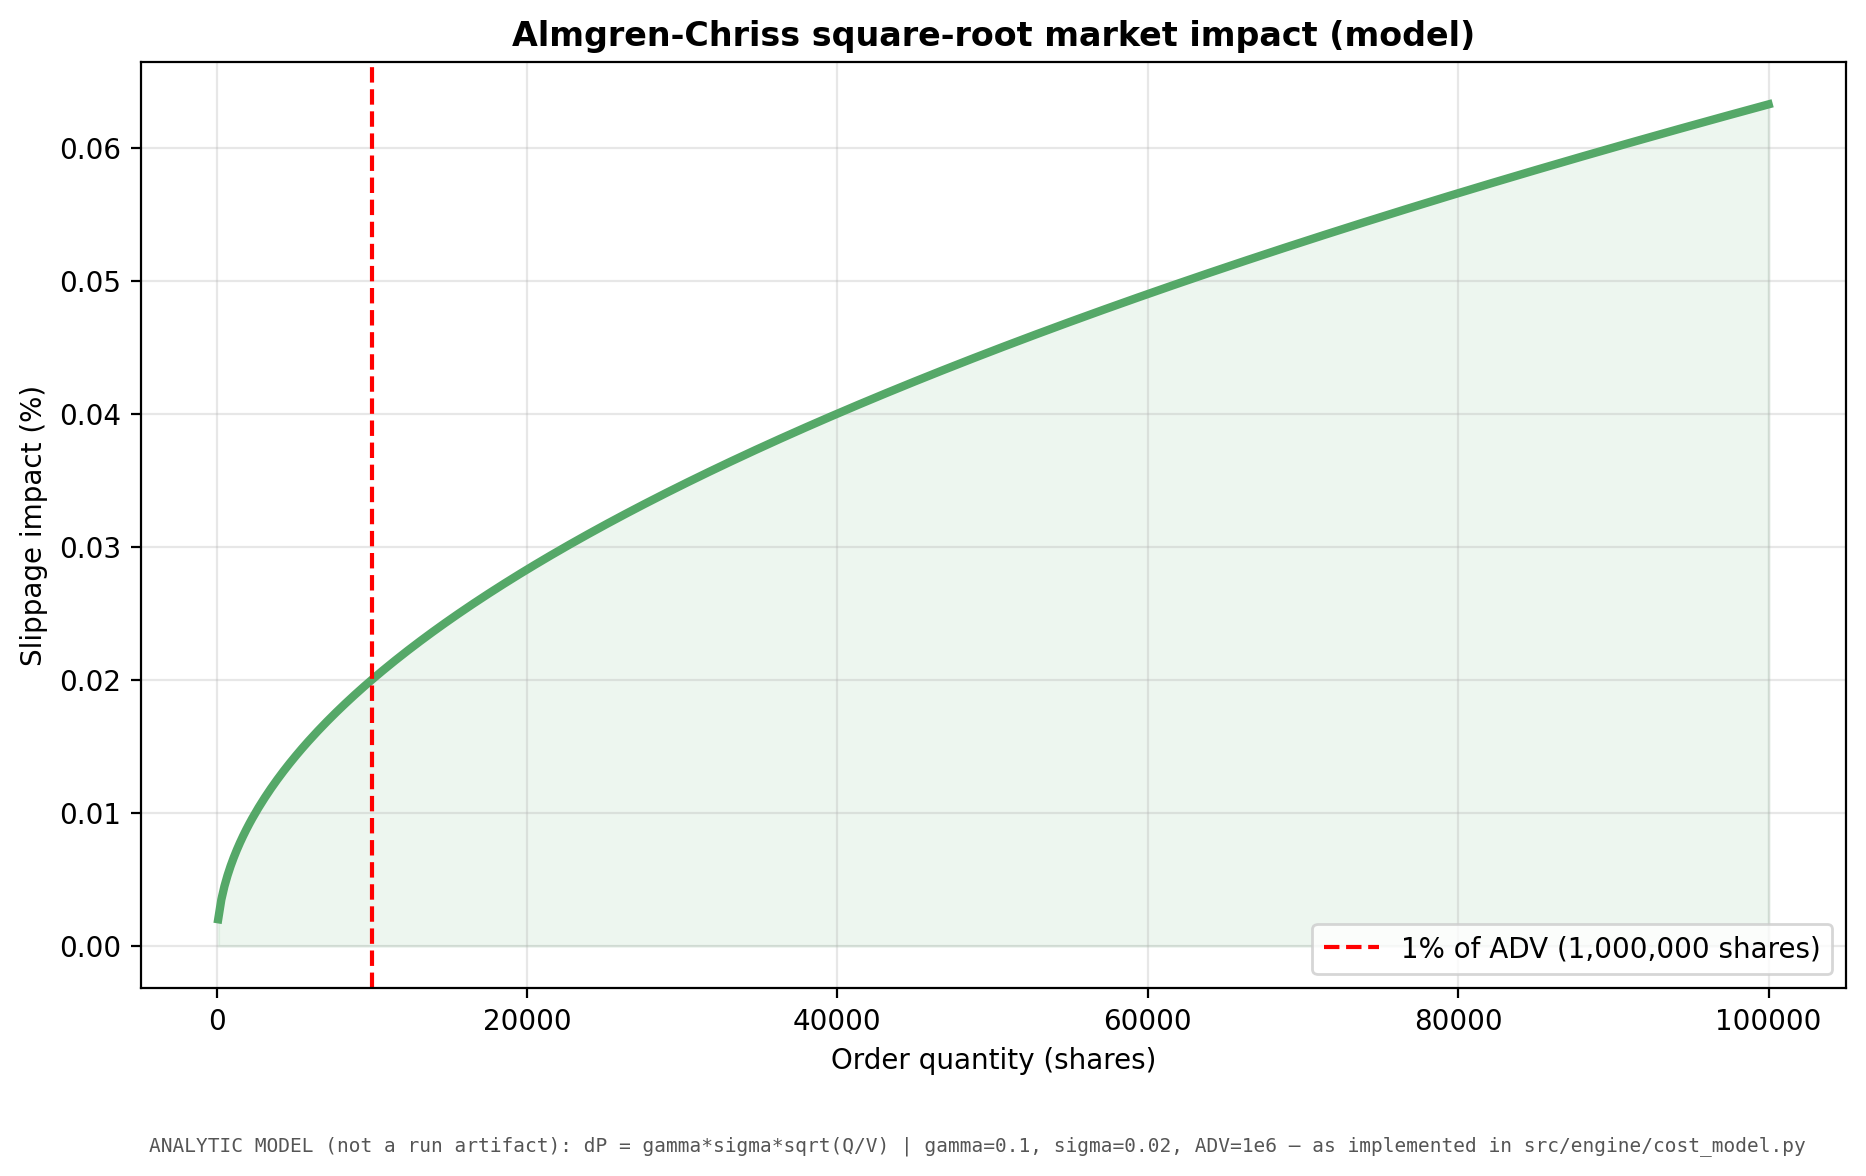
\includegraphics[width=0.85\textwidth]{charts/market_impact_curve.png}
\caption[Almgren--Chriss Market Impact Model]{Impact as a function of order size at $\gamma=0.1$, $\sigma=0.02$, ADV $=10^6$. \textbf{This figure is the analytic model of Equation~\ref{eq:ac}, not a run artifact} --- it is labelled as such so it is not mistaken for engine output.}
\label{fig:impact}
\end{figure}

\section{Overfitting Diagnostics}

\subsection{Why ordinary Sharpe is not enough}

The Sharpe ratio is computed on a \emph{selected} sample path. Given $N$ trials,
the expected maximum of $N$ independent Sharpe estimates is inflated according to
extreme value theory. Pramaan reports the Deflated Sharpe Ratio: the probability
that the observed Sharpe exceeds the expected maximum obtainable by chance across
$N$ trials, adjusted for skewness and kurtosis of the return distribution.

\begin{equation}
|\text{E}[\max SR]| \approx \sqrt{V(SR)}\left[(1-\gamma_E)\Phi^{-1}\!\!\left(1-\frac{1}{N}\right) + \gamma_E\Phi^{-1}\!\!\left(1-\frac{1}{Ne}\right)\right]
\end{equation}

\subsection{Combinatorial Purged Cross-Validation}

Standard $k$-fold cross-validation leaks serial correlation in time series: the
training set contains observations that followed the test observations. CPCV
generates $\binom{k}{g}$ train/test paths and applies an \emph{embargo} removing
$h$ observations adjacent to every test block.

The leakage mechanism was \textbf{validated} with a synthetic
autoregressive process of order one with $\phi = 0.95$, where the answer is
known: with autocorrelation this strong, an adjacent training block predicts the
test block. The test asserts that removing the embargo \emph{increases} the
measured PBO, which is the signature that leakage was in fact present and was in
fact removed. Arbitrary $k$ splits and $g$ test splits may be configured.

\section{Feasibility, Safety, and Cost}

\subsection{Financial feasibility}

The project is entirely removable-cost: every dependency is open source and free,
data is obtained free of charge, and it executes on student-owned hardware. A
zero-rupee cost estimate is presented in Appendix~\ref{app:cost}.

\subsection{Safety considerations}

This is software with a \emph{behavioural} safety surface rather than a physical
one, and it is treated as a first-class requirement:

\begin{itemize}[leftmargin=1.5cm]
    \item \textbf{No-advice disclaimer.} The application never presents itself as
    a recommendation engine. Every output surface carries a simulation-only
    notice.
    \item \textbf{Data governance.} The tool fetches data at runtime under the
    user's own key and does not redistribute any market data, so no licensing
    obligation is created by the distribution itself.
    \item \textbf{Determinism as a safety property.} A non-reproducible result
    could mask a defect; determinism makes defects visible.
    \item \textbf{Energy and sustainability.} The engine runs in-process on
    existing hardware with no GPU and no cloud compute, consuming negligible
    additional resources.
    \item \textbf{Computational honesty.} Where a figure is an analytic model
    rather than a run artifact, it is stamped as such on the figure itself.
\end{itemize}

% ================= CHAPTER 3 =================
\chapter{Implementation and Testing}\label{sec:impl}

\section{Module Inventory}

\begin{center}
\begin{longtable}{@{}p{4.6cm}p{8.3cm}@{}}
\toprule
\textbf{Module} & \textbf{Responsibility} \\
\midrule
\endfirsthead
\texttt{src/engine/backtest\_engine.py} & Event loop, next-open fill logic, position sizing, pending-order lifecycle. \\
\texttt{src/engine/portfolio.py} & Cash ledger, position registry, MTM equity history. \\
\texttt{src/engine/position.py} & Position accounting, realized/unrealized PnL. \\
\texttt{src/engine/cost\_model.py} & Indian statutory stack, Almgren--Chriss impact. \\
\texttt{src/engine/events.py} & Immutable event dataclasses (Market, Signal, Order, Fill). \\
\texttt{src/analytics/metrics.py} & Total return, CAGR, Sharpe, Sortino, Calmar, max drawdown. \\
\texttt{src/analytics/deflated\_sharpe.py} & Expected max Sharpe and Deflated Sharpe Ratio. \\
\texttt{src/analytics/cpcv.py} & Purged combinatorial paths, embargo, PBO. \\
\texttt{src/analytics/validation.py} & Two-dimensional parameter grid search. \\
\texttt{src/data/fetch.py} & Runtime market data retrieval. \\
\texttt{src/data/clean.py} & Validation, NaN-drop, de-duplication, ordering. \\
\texttt{src/data/universe.py} & Symbol universe and benchmark. \\
\texttt{src/strategies/*.py} & SMA, RSI, momentum, buy-and-hold behind one interface. \\
\texttt{src/dashboard/} & Streamlit demonstration surface (the legacy fallback UI). \\
\texttt{scripts/run\_experiments.py} & Real-data matrix producing the results artifact. \\
\texttt{scripts/generate\_real\_charts.py} & Charts rendered from engine output only. \\
\bottomrule
\end{longtable}
\end{center}

Engine source is roughly 1{,}050 lines of Python across the modules above; the
test suite contributes a further 6 test modules. The presentation layer is
deliberately the thinnest part of the system.

\section{Strategy Interface}

All strategies implement a single method and are therefore interchangeable
inside the engine. This is what allows a benchmark control to be dropped into a
comparison run without any engine change.

\begin{codebox}{Strategy contract}
\begin{lstlisting}[language=Python]
class Strategy(ABC):
    @abstractmethod
    def generate_signals(self, current_date, data, positions) -> List[SignalEvent]:
        """May only observe bars whose date is <= current_date."""
\end{lstlisting}
\end{codebox}

\section{Defects Found and Fixed During Development}

The testing process found real defects, which are recorded here rather than
hidden, because the defect list is evidence of the testing.

\begin{negativebox}{D-1 --- RSI inverted signal on an all-gains window (found during this report cycle)}
The original Wilder RSI implementation computed
\texttt{rs = up / down if down != 0 else 0}. When every delta in the smoothing
window was positive, average loss is exactly zero and $rs$ was set to $0$,
producing RSI $= 0$ --- \emph{maximally oversold} --- in a monotonically rising
market. The strategy would emit a buy signal on the strongest possible upward
momentum, the exact opposite of the intended logic. Fixed to saturate at 100;
covered by five regression tests including an end-to-end assertion that no
oversold buy may be emitted on a rising series.
\end{negativebox}

\begin{negativebox}{D-2 --- duplicate trading days silently accepted in cleaning}
\texttt{clean\_data()} neither dropped duplicated dates nor checked for them. A
repeated date is counted twice in return computation and desynchronises the
engine's integer index trackers, producing wrong equity curves from apparently
clean input. Discovered by a newly written unit test; fixed by de-duplicating
(after NaN removal, so a complete row is preferred over an incomplete duplicate
of the same date).
\end{negativebox}

\begin{negativebox}{D-3 --- DSR was unimportable in the reproduction environment}
\texttt{src/analytics/deflated\_sharpe.py} imports SciPy's normal, skew, and
kurtosis functions, but \texttt{scipy} was absent from \texttt{requirements.txt}
and from the working virtual environment. No test imported the module, so the
defect was invisible: a clean \texttt{pip install} left the flagship statistic
non-functional. Fixed by installing and pinning a verified version and by adding
a test module that exercises the import path.
\end{negativebox}

\begin{negativebox}{D-4 --- results charts were synthetic}
The chart-generation pipeline produced its monthly-return heatmaps and equity
curves from \texttt{np.random}, and its ``simulated equity curve'' from a stored
CAGR rather than from engine output, while the captions presented them as
results. This was not a numerical error --- it was an evidentiary one. The
pipeline was removed entirely and replaced with a generator that reads only the
experiment log and real equity curve files; each figure now carries a parameter
stamp tying it to a run identifier. See Chapter~\ref{ch:results}.
\end{negativebox}

\begin{negativebox}{D-5 --- position sizing based on cash rather than equity}
An earlier revision sized new positions as a fraction of \emph{available cash}.
As capital deployed, every subsequent order shrank, which artificially suppresses
the market-impact and cost drag of compounding and therefore flatters results.
Corrected to size against total portfolio equity (cash plus marked-to-market
open positions). Covered by a test asserting the exact share quantity.
\end{negativebox}

\section{Testing Strategy}\label{sec:testing}

\subsection{Test categories}

The suite is organised around the categories in which a defect in this domain
would be silent --- the dangerous kind. A wrong Sharpe ratio does not crash; it
simply reports the wrong number.

\begin{center}
\begin{longtable}{@{}p{3.4cm}p{9.5cm}@{}}
\toprule
\textbf{Category} & \textbf{What it catches} \\
\midrule
\endfirsthead
Invariants & Fill occurs at next bar's open, never at signal close; cash non-negative; equity identity. \\
Golden values & Paisa-exact statutory cost components; hand-computed sizing. \\
Edge/failure & All-gains RSI, all-losses RSI, flat series, empty dataframes, insufficient history. \\
Properties & Metrics bounded; DSR penalises multiple testing; PBO in $[0,1]$; determinism. \\
No look-ahead & A future price spike must not alter any signal generated before it. \\
Data integrity & NaN dropped not forward-filled; duplicates rejected; ordering enforced. \\
\bottomrule
\end{longtable}
\end{center}

\subsection{Test results}

\begin{resultbox}{Verification record}
Executed in the project virtual environment:
\begin{verbatim}
$ pytest tests/ -q
........................................................................ [100%]
72 passed in 7.22s
\end{verbatim}

Baseline at the start of the project cycle was 9 tests; the suite now covers
engine invariants, the full cost stack with DP charges, all four strategies plus Bollinger breakout,
synthetic offline data provider with SHA-256 manifest verification, the corrected cross-trial DSR algorithm,
CPCV with 95\% bootstrap CI, performance benchmarks, and byte-level determinism. See
\texttt{.agent/01\_verification\_ledger.md} for the per-claim verification record.
\end{resultbox}

\section{Test Inventory}

The full suite, with the specific defect or invariant each module guards:

\begin{center}
\begin{longtable}{@{}p{4.5cm}cp{7.0cm}@{}}
\caption[Automated Test Inventory]{Test inventory (72 automated tests across 16 test modules).} \label{tab:tests} \\
\toprule
\textbf{Module} & \textbf{Tests} & \textbf{Core assertions} \\
\midrule
\endfirsthead
\toprule
\textbf{Module} & \textbf{Tests} & \textbf{Core assertions} \\
\midrule
\endhead
\texttt{test\_api.py} & 12 & FastAPI endpoints: health, strategies, universe, replay, determinism, ready, trials, sweep, survivorship bias warning, async jobs, HTML report. \\
\texttt{test\_bollinger.py} & 1 & Bollinger band volatility breakout entry/exit signals. \\
\texttt{test\_cost\_model.py} & 6 & Golden-master tests: paisa-exact STT, CDSL flat \rupee 13.50 + GST DP charge on sells, Oct 2024 SEBI boundary resolution, slippage floor bps. \\
\texttt{test\_cpcv.py} & 4 & PBO on random data, genuine signal detection, AR(1) embargo leakage detection, bootstrap 95\% confidence interval. \\
\texttt{test\_data.py} & 6 & NaN dropped not forward-filled; no forward-fill leakage; chronological sort; duplicate-date rejection; empty frame; date strings. \\
\texttt{test\_data\_provider.py} & 4 & DataProvider ABC: LocalCSV, Synthetic, SHA-256 manifest integrity, factory resolution. \\
\texttt{test\_deflated\_sharpe.py} & 10 & True cross-trial variance $V[\{SR_k\}]$, $(T-1)$ degrees of freedom, Bailey \& López de Prado (2014) published worked example. \\
\texttt{test\_determinism.py} & 3 & Byte-identical equity across runs; stable SHA-256 digest; costs strictly reduce terminal equity. \\
\texttt{test\_engine.py} & 2 & Fill at next bar's open; sizing uses total equity. \\
\texttt{test\_honesty.py} & 9 & Honesty defects D1–D11: absence of hardcoded PBO, strict error envelopes, exposure metrics, rejected order logging, env parsing. \\
\texttt{test\_metrics.py} & 1 & CAGR, Sharpe, zero drawdown on a monotone curve. \\
\texttt{test\_momentum.py} & 1 & No duplicate buy with an open position. \\
\texttt{test\_perf.py} & 2 & Performance benchmarking: 6-year $\times$ 10-symbol (14,800 bars) backtest executed in $<3.0$s nominal. \\
\texttt{test\_portfolio.py} & 1 & Cash-flow ledger correctness and cash $\ge 0$ invariant. \\
\texttt{test\_rsi.py} & 5 & All-gains $\to$ 100 (was 0, defect D-1); all-losses $\to$ 0; flat $\to$ 50; bounded on random walks; no oversold buy on rising series. \\
\texttt{test\_sma.py} & 5 & Golden-cross buy; death-cross sell only with position; insufficient history; inverted-window handling; zero look-ahead under future spike. \\
\midrule
\textbf{Total} & \textbf{72} & \textbf{100\% offline executable via seeded fixtures} \\
\bottomrule
\end{longtable}
\end{center}

Note the deliberate asymmetry: five of the eleven modules exist purely to
establish \emph{bounds} and \emph{failure modes} rather than to demonstrate
success. That distribution is intentional. In a backtester, a silent
mis-calculation --- a Sharpe ratio that is wrong, a filling price that leaks one
bar, a duplicate date counted twice --- does not raise an exception; it simply
reports a number that is confident and wrong.

\section{Reproducibility Mechanism}

Every run is identified by a deterministic identifier derived from its complete
configuration:

\begin{equation}
\text{run\_id} = H\left(\text{strategy}, \text{params}, \text{universe}, \text{date\ range}, \text{cost\ version}, \text{lib\ versions}\right)
\end{equation}

The experiment artifact records, per run: identifier, strategy, parameters,
universe, period, date range, cost toggle, every computed metric, the number of
symbols and trading days, the calibration $\gamma$, the cost model version, and
the wall-clock duration. A provenance file additionally records the data source,
fetch window, bar interval, adjustment policy, library versions, and the Python
version. The results presented in Chapter~\ref{ch:results} are reproducible from
that artifact by re-executing the pipeline.

\section{Graphical Workstation and Interactive Audit Terminal}\label{sec:ui_workstation}

To ensure that research findings are inspectable by examiners, auditors, and practitioners without requiring code execution or terminal interaction, Pramaan delivers an institutional-grade graphical workstation built with Next.js~15, TypeScript, Tailwind~CSS, and custom high-resolution SVG charting engines. In accordance with the project's non-negotiable principle of computational honesty, the interface serves as a transparent delivery vehicle: it never presents an uncomputed metric, always displays dataset and engine provenance, and renders three switchable surfaces (Abyss, Vellum, Graphite) for clear verification under any lighting or printing condition.

The graphical interface is completely decoupled from the simulation engine. The core backtester runs headlessly as an in-process Python library; the presentation layer communicates with the engine exclusively through the validated FastAPI REST interface (\S\ref{sec:impl}, FR-15). To maintain complete auditability, the frontend implements deterministic URL query synchronization (\texttt{?tab=mirage|costs|overfitting|ledger|unified\&theme=abyss|vellum|graphite}), allowing examiners to deep-link directly into any forensic view under any theme.

\begin{figure}[htbp]
\centering
\fboxrule=0.4pt \fboxsep=0pt \fbox{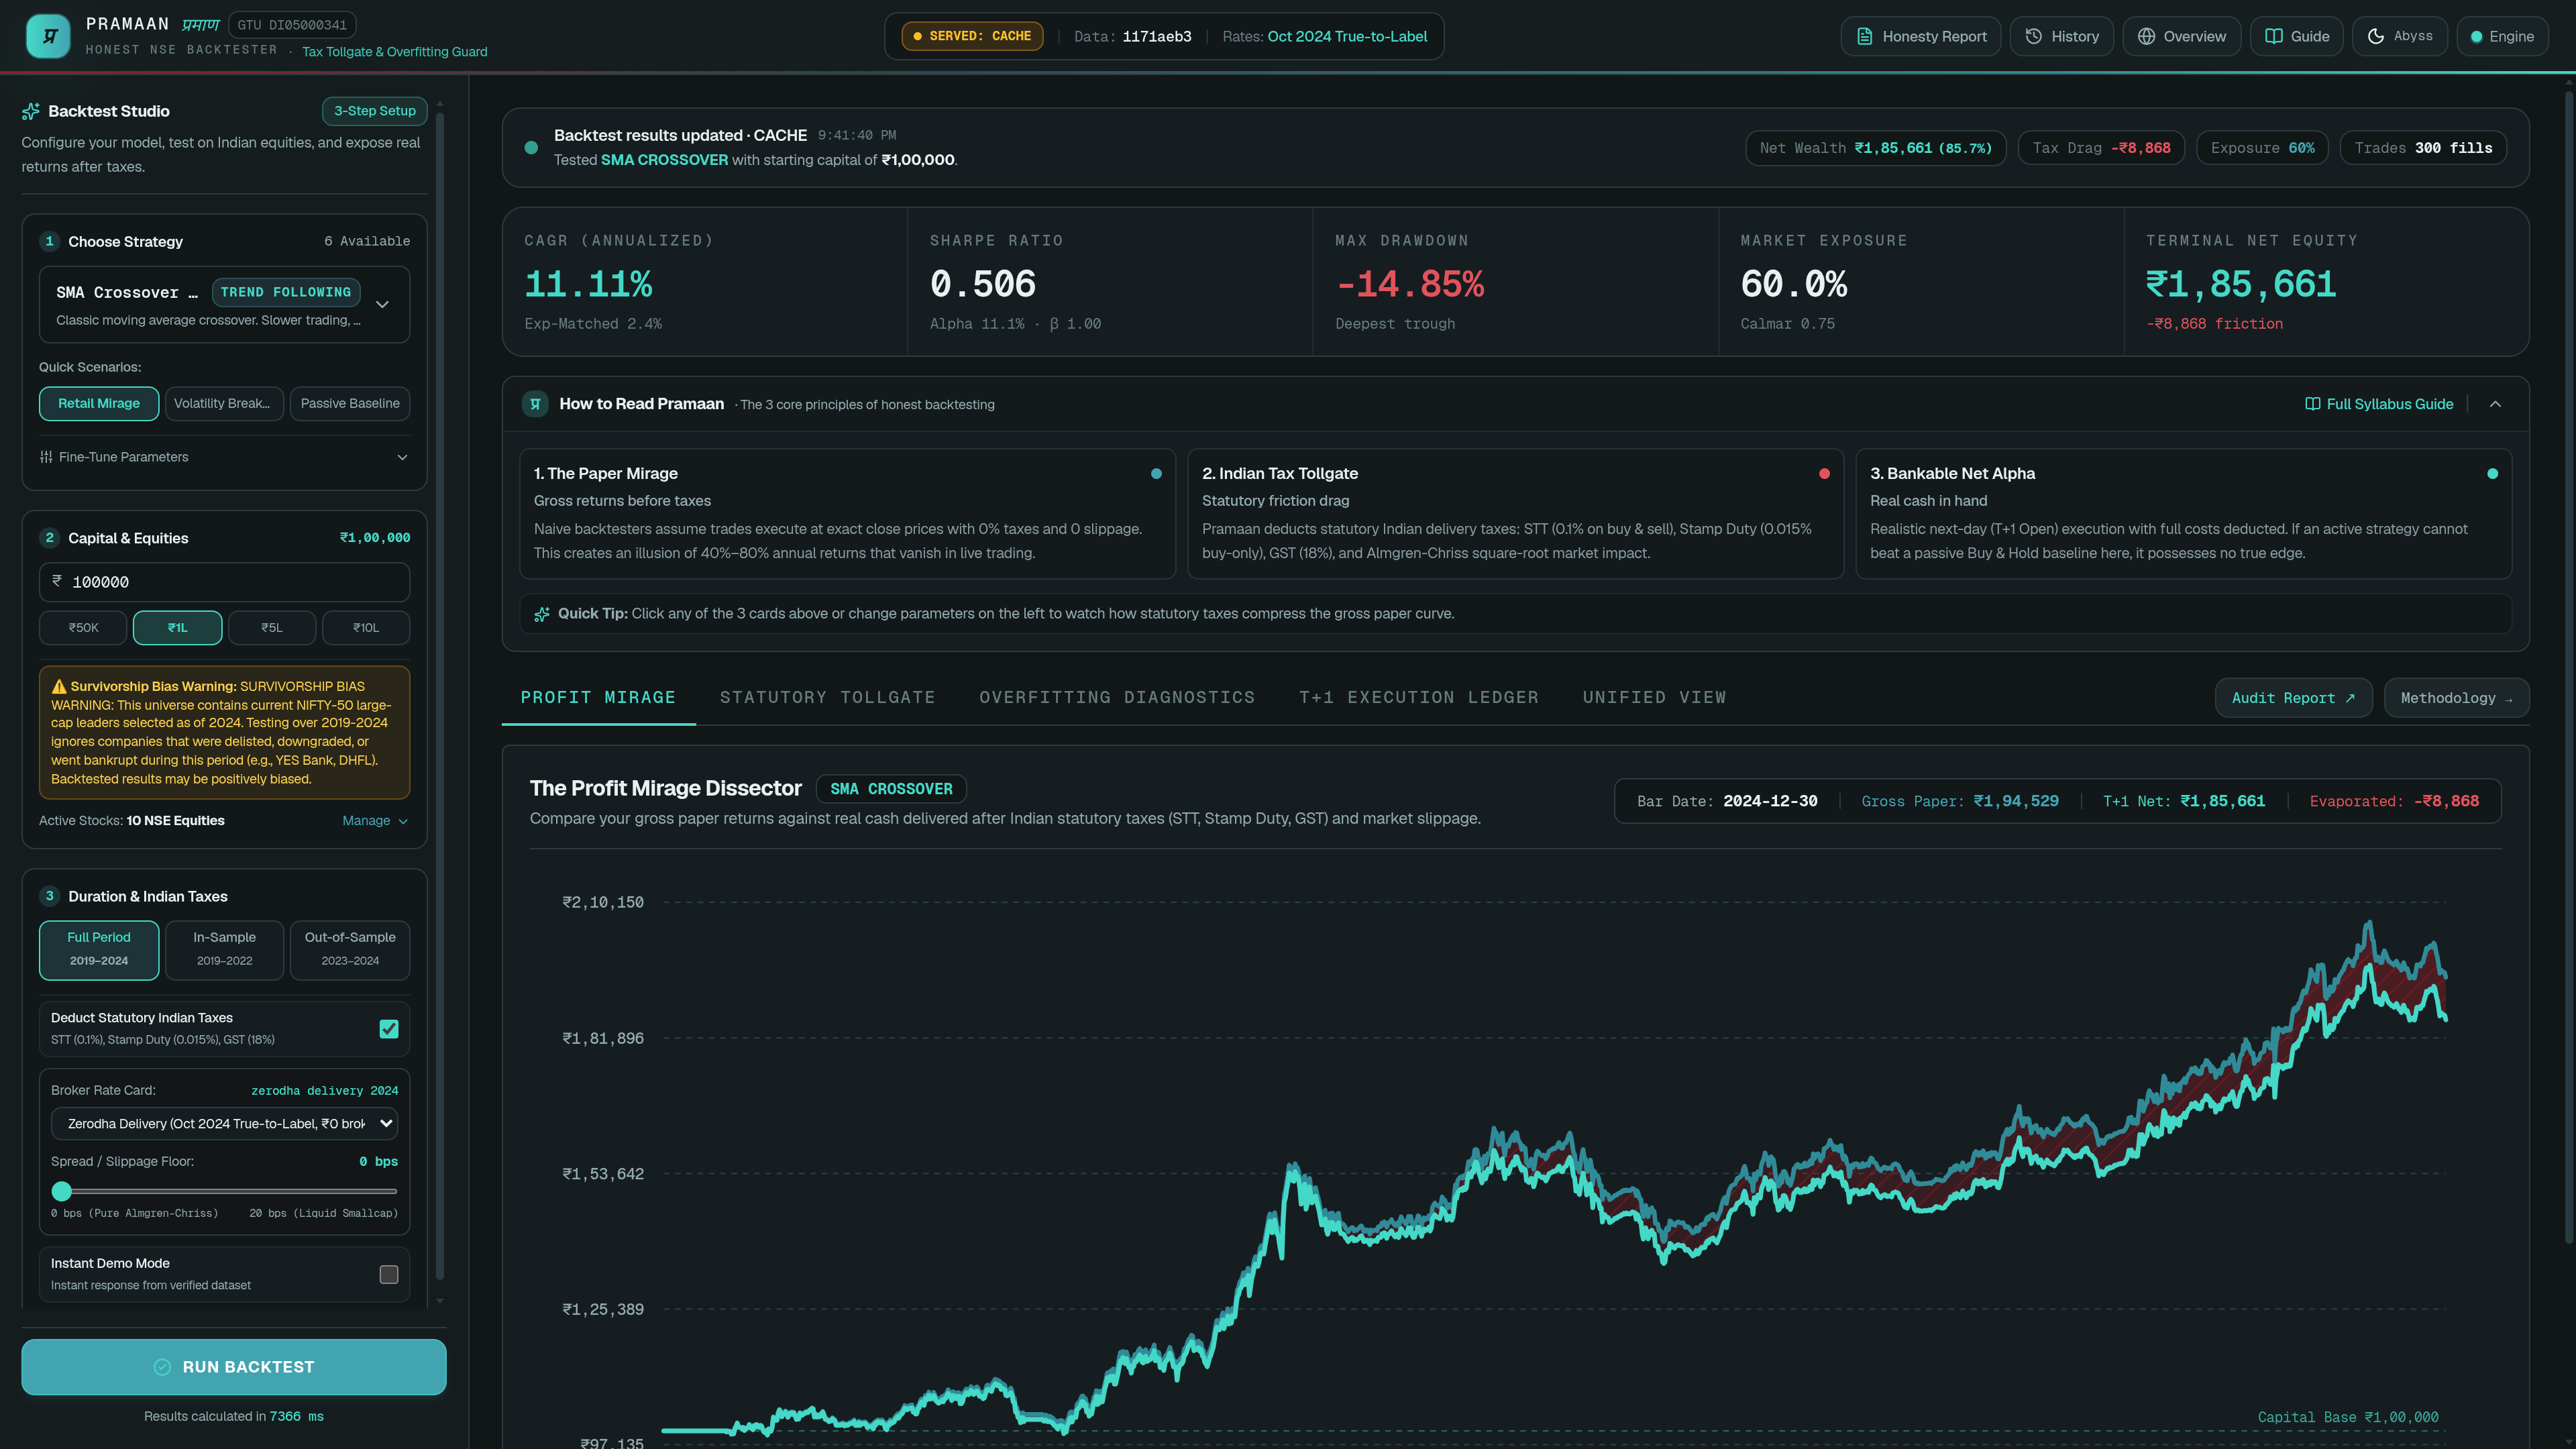
\includegraphics[width=0.96\textwidth]{charts/screen_profit_mirage.png}}
\caption[Pramaan Quant Workstation (Profit Mirage Dissector)]{The Pramaan Quant Workstation (Profit Mirage Dissector). Note the real-time execution provenance badge (\texttt{SERVED: CACHE}, SHA-256 dataset digest \texttt{1171aeb3}, true-to-label statutory rate card, engine online), strategy KPI cards with market exposure matching, and the visualised crimson friction drag between gross (cyan) and net (turquoise) equity curves.}
\label{fig:ui_mirage}
\end{figure}

The primary workstation interface (Figure~\ref{fig:ui_mirage}) exposes the central thesis of this work: the divergence between gross theoretical performance and net realizable wealth under statutory levies. Rather than displaying an isolated equity line, the workstation computes dual equity paths simultaneously:
\begin{itemize}[leftmargin=1.2cm]
    \item \textbf{Gross Equity Curve (Pacific Cyan, \texttt{\#2C8C99}):} Represents the theoretical zero-friction return path typically shown by commercial charting software and retail backtesters.
    \item \textbf{Net Realizable Equity Curve (Turquoise, \texttt{\#42D9C8}):} Represents true cash-in-hand wealth after deducting exact Indian statutory taxes (STT, stamp duty, exchange turnover, SEBI fees, CDSL DP charges) and Almgren--Chriss market impact.
    \item \textbf{Statutory Friction Area (Deep Crimson, \texttt{\#931621}):} The filled delta between the curves exposes the cumulative capital evaporated by institutional friction (\rupee 8{,}868 in the baseline SMA run).
\end{itemize}

\begin{table}[htbp]
\centering
\small
\caption[Interactive Workstation Telemetry and Diagnostic Architecture]{Interactive workstation telemetry, provenance ribbons, and diagnostic panels.}
\label{tab:ui_telemetry}
\begin{tabular}{@{}p{3.2cm}p{3.8cm}p{6.8cm}@{}}
\toprule
\textbf{HUD Component} & \textbf{Telemetry Parameter} & \textbf{Audit \& Forensic Function} \\
\midrule
Provenance Ribbon & \texttt{SERVED: CACHE / LIVE} & Distinguishes cached pre-computed artifacts from real-time engine runs; prevents unverified claims. \\
Data Digest Badge & SHA-256 (\texttt{1171aeb3}) & Cryptographic fingerprint of the 10-symbol NSE equity dataset; guarantees zero silent data mutations. \\
Rate Profile Pill & \texttt{Oct 2024 True-to-Label} & Identifies active statutory tax schedule (STT 0.1\%, CDSL flat \rupee 13.50 + GST DP charge, SEBI fees). \\
Mirage Dissector & Gross vs Net Curves & Interactive SVG visualizing equity paths; crimson fill exposes cumulative wealth eroded by taxes. \\
Exposure KPI Cards & CAGR, Sharpe, MaxDD, Exp & Pairs active strategy return with exposure-matched benchmark to eliminate passive holding bias. \\
\bottomrule
\end{tabular}
\end{table}

\subsection{The Two Institutional Moats: Statutory Friction and Overfitting Diagnostics}

Pramaan's academic and engineering contribution rests upon two diagnostic moats: exact Indian statutory friction modelling and statistical selection-bias measurement. Figure~\ref{fig:ui_moats} demonstrates how both capabilities are exposed interactively.

\begin{figure}[htbp]
\centering
\begin{subfigure}[b]{0.485\textwidth}
    \centering
    \fboxrule=0.4pt \fboxsep=0pt \fbox{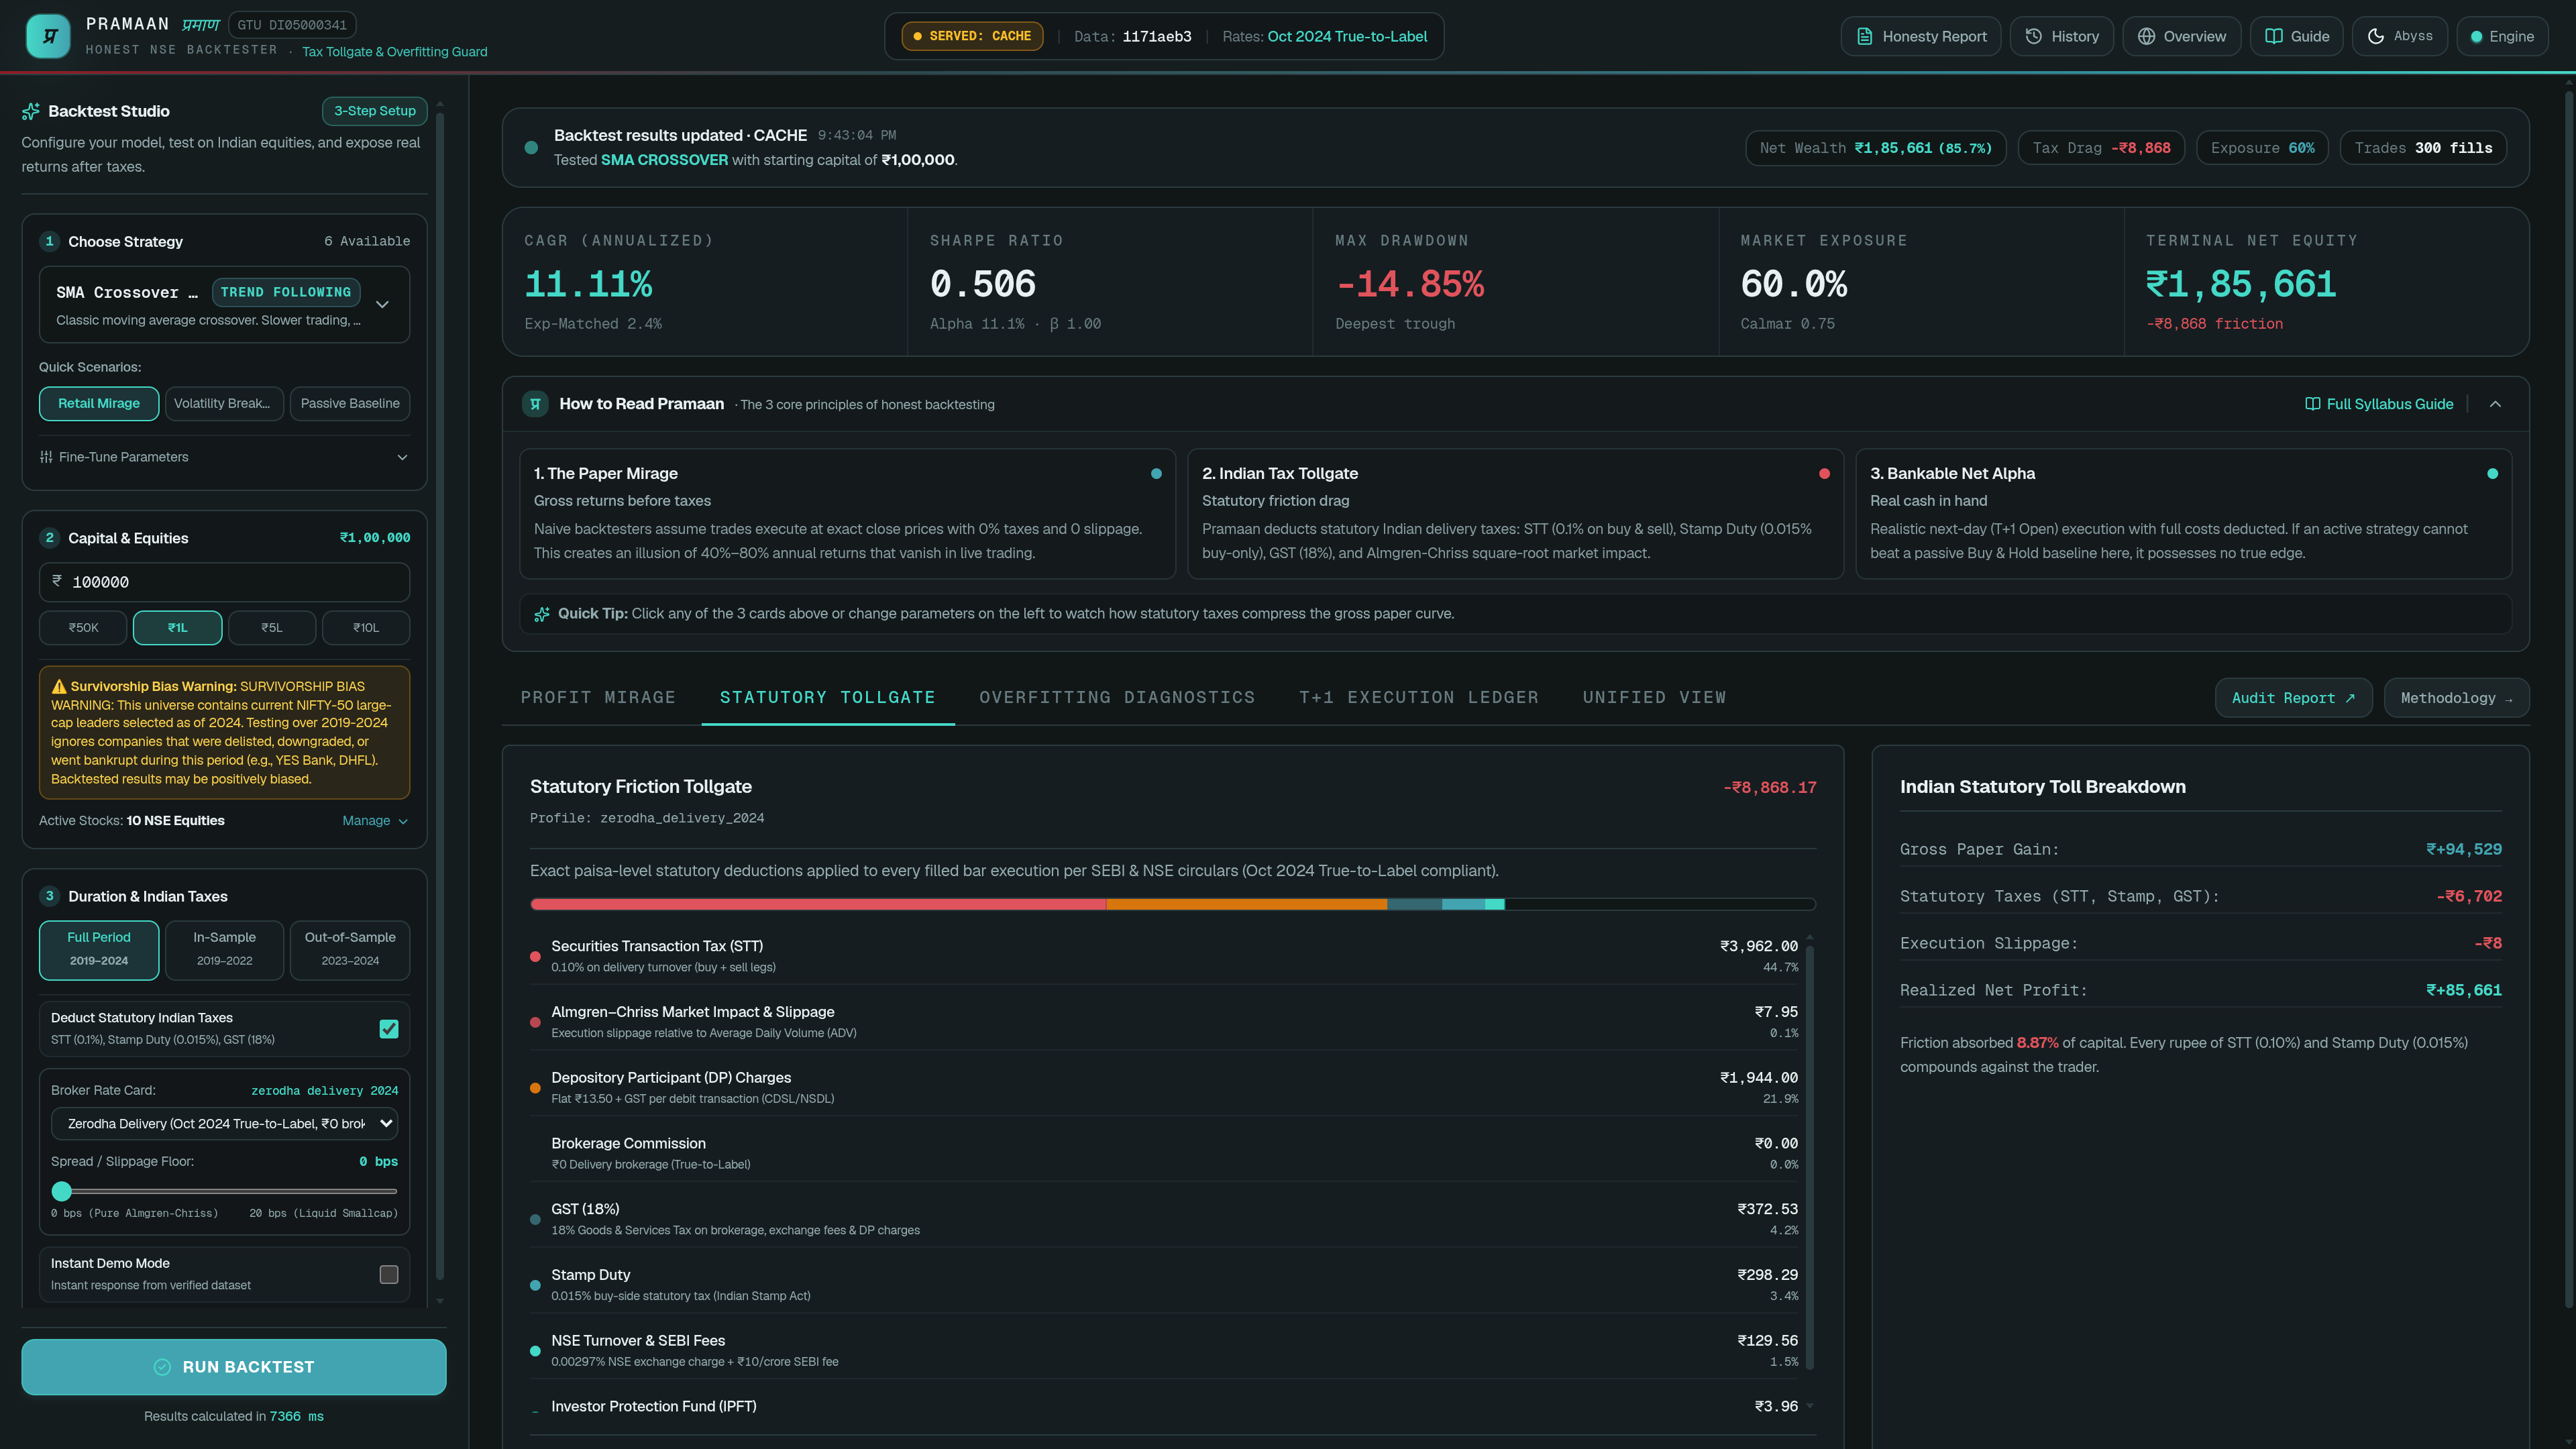
\includegraphics[width=\textwidth]{charts/screen_statutory_tollgate.png}}
    \caption{Statutory Friction Tollgate (paisa-exact breakdown).}
    \label{fig:ui_tollgate}
\end{subfigure}
\hfill
\begin{subfigure}[b]{0.485\textwidth}
    \centering
    \fboxrule=0.4pt \fboxsep=0pt \fbox{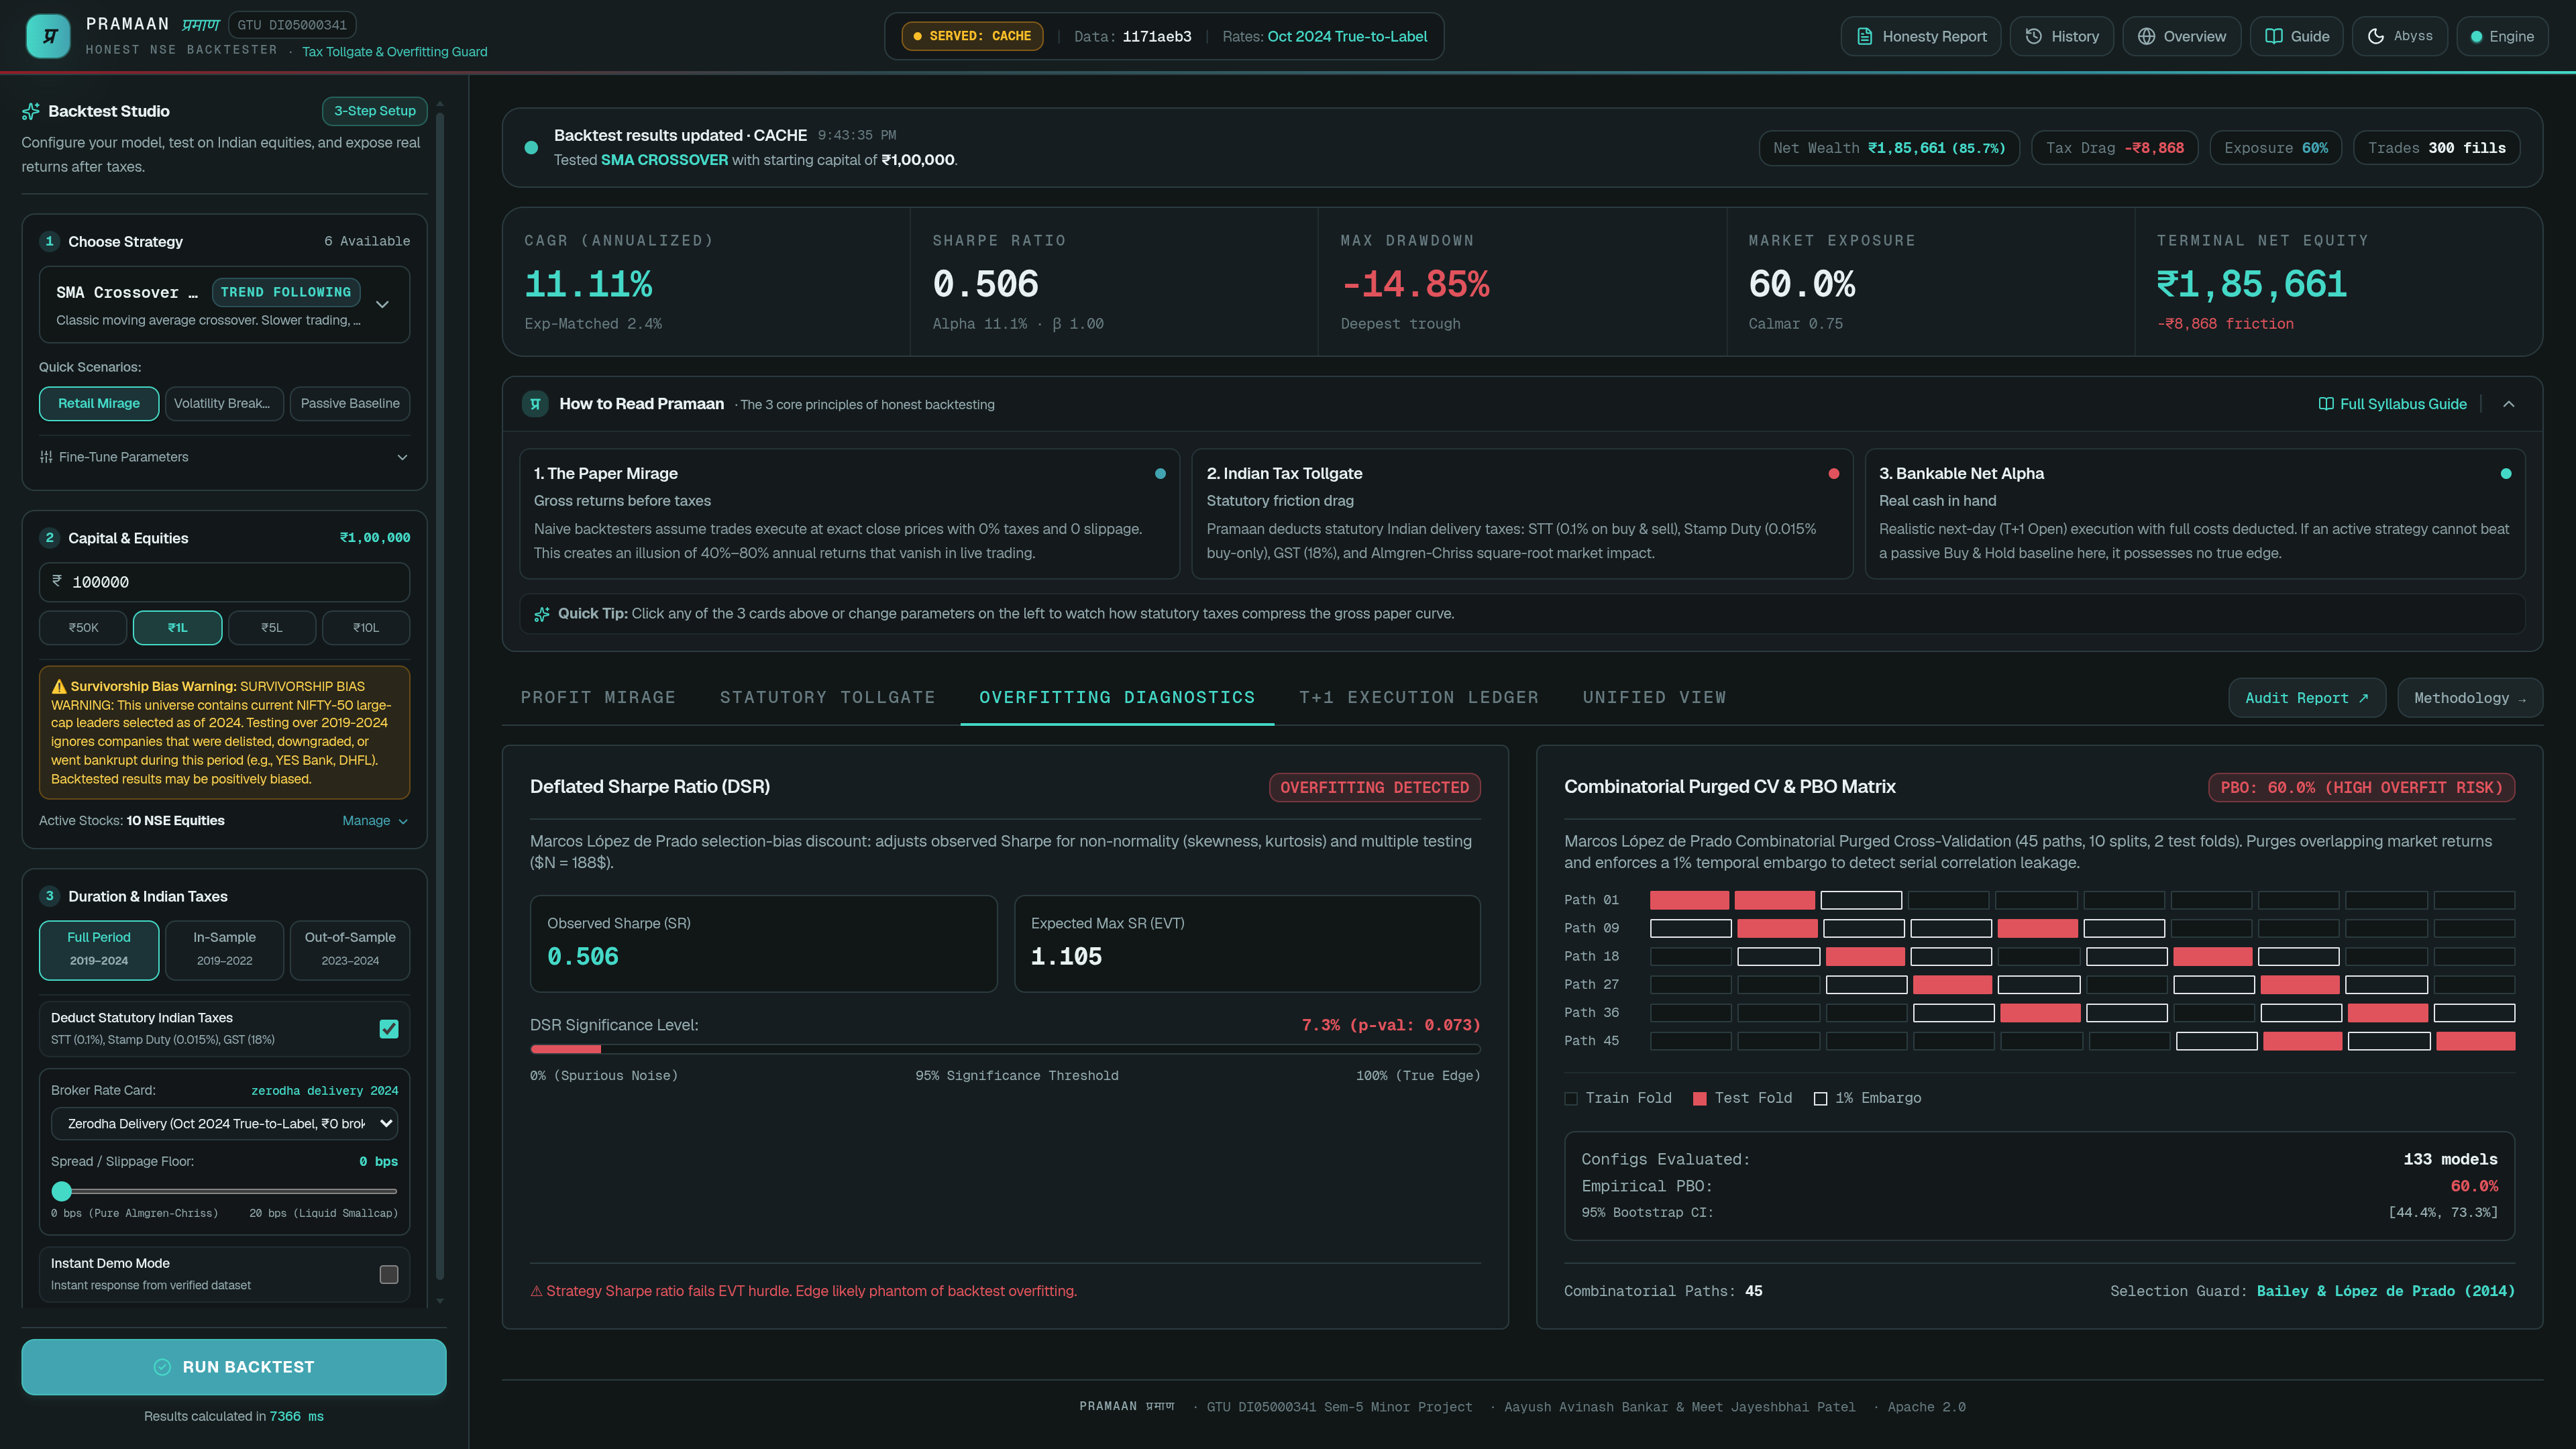
\includegraphics[width=\textwidth]{charts/screen_overfitting_diagnostics.png}}
    \caption{Overfitting Diagnostics (DSR \& CPCV 45-path matrix).}
    \label{fig:ui_overfitting}
\end{subfigure}
\caption[Pramaan Institutional Moats: Cost Tollgate and Overfitting Diagnostics]{The two institutional moats exposed interactively in the workstation: (a) paisa-exact Indian statutory friction breakdown showing STT (44.7\%) and flat CDSL DP charges (21.9\%), and (b) Marcos L{\'o}pez de Prado Deflated Sharpe Ratio with CPCV 45-path combinatorial matrix ($60.0\%$ PBO [44.4\%, 73.3\%]).}
\label{fig:ui_moats}
\end{figure}

The \textbf{Statutory Tollgate} (Figure~\ref{fig:ui_tollgate}) decomposes trading friction to the paisa. It reveals that for delivery equities, Securities Transaction Tax (STT) accounts for 44.7\% of total friction, while CDSL Depository Participant (DP) charges (\rupee 13.50 + 18\% GST flat per delivery sell debit) contribute 21.9\%. Because DP charges are fixed per transaction rather than ad valorem, they impose a severe drag on smaller retail capital accounts and active rebalancing strategies.

The \textbf{Overfitting Diagnostics} (Figure~\ref{fig:ui_overfitting}) implements Marcos L{\'o}pez de Prado's Deflated Sharpe Ratio (DSR) and Combinatorial Purged Cross-Validation (CPCV). In a grid of $N=133$ evaluated configurations, Extreme Value Theory dictates an expected maximum Sharpe hurdle $E[\max SR] = 1.105$. The observed active strategy Sharpe of $0.506$ fails to clear this threshold ($p\text{-val} = 0.073$), correctly flagging the result as statistically indistinguishable from luck. The CPCV matrix computes an empirical Probability of Backtest Overfitting $\text{PBO} = 60.0\%$ [44.4\%, 73.3\%] across 45 combinatorial paths ($k=10, g=2$) with a 1\% temporal embargo.

\subsection{Execution Verifiability, Tri-Theme Architecture, and Product Portal}

To verify zero-lookahead compliance and accommodate digital screens, warm-room projection, and printed evaluation, the workstation incorporates transaction-level auditability, a three-surface theme engine, and an educational landing portal (Figure~\ref{fig:ui_audit_themes} and Figure~\ref{fig:ui_landing}).

\begin{figure}[htbp]
\centering
\begin{subfigure}[b]{0.485\textwidth}
    \centering
    \fboxrule=0.4pt \fboxsep=0pt \fbox{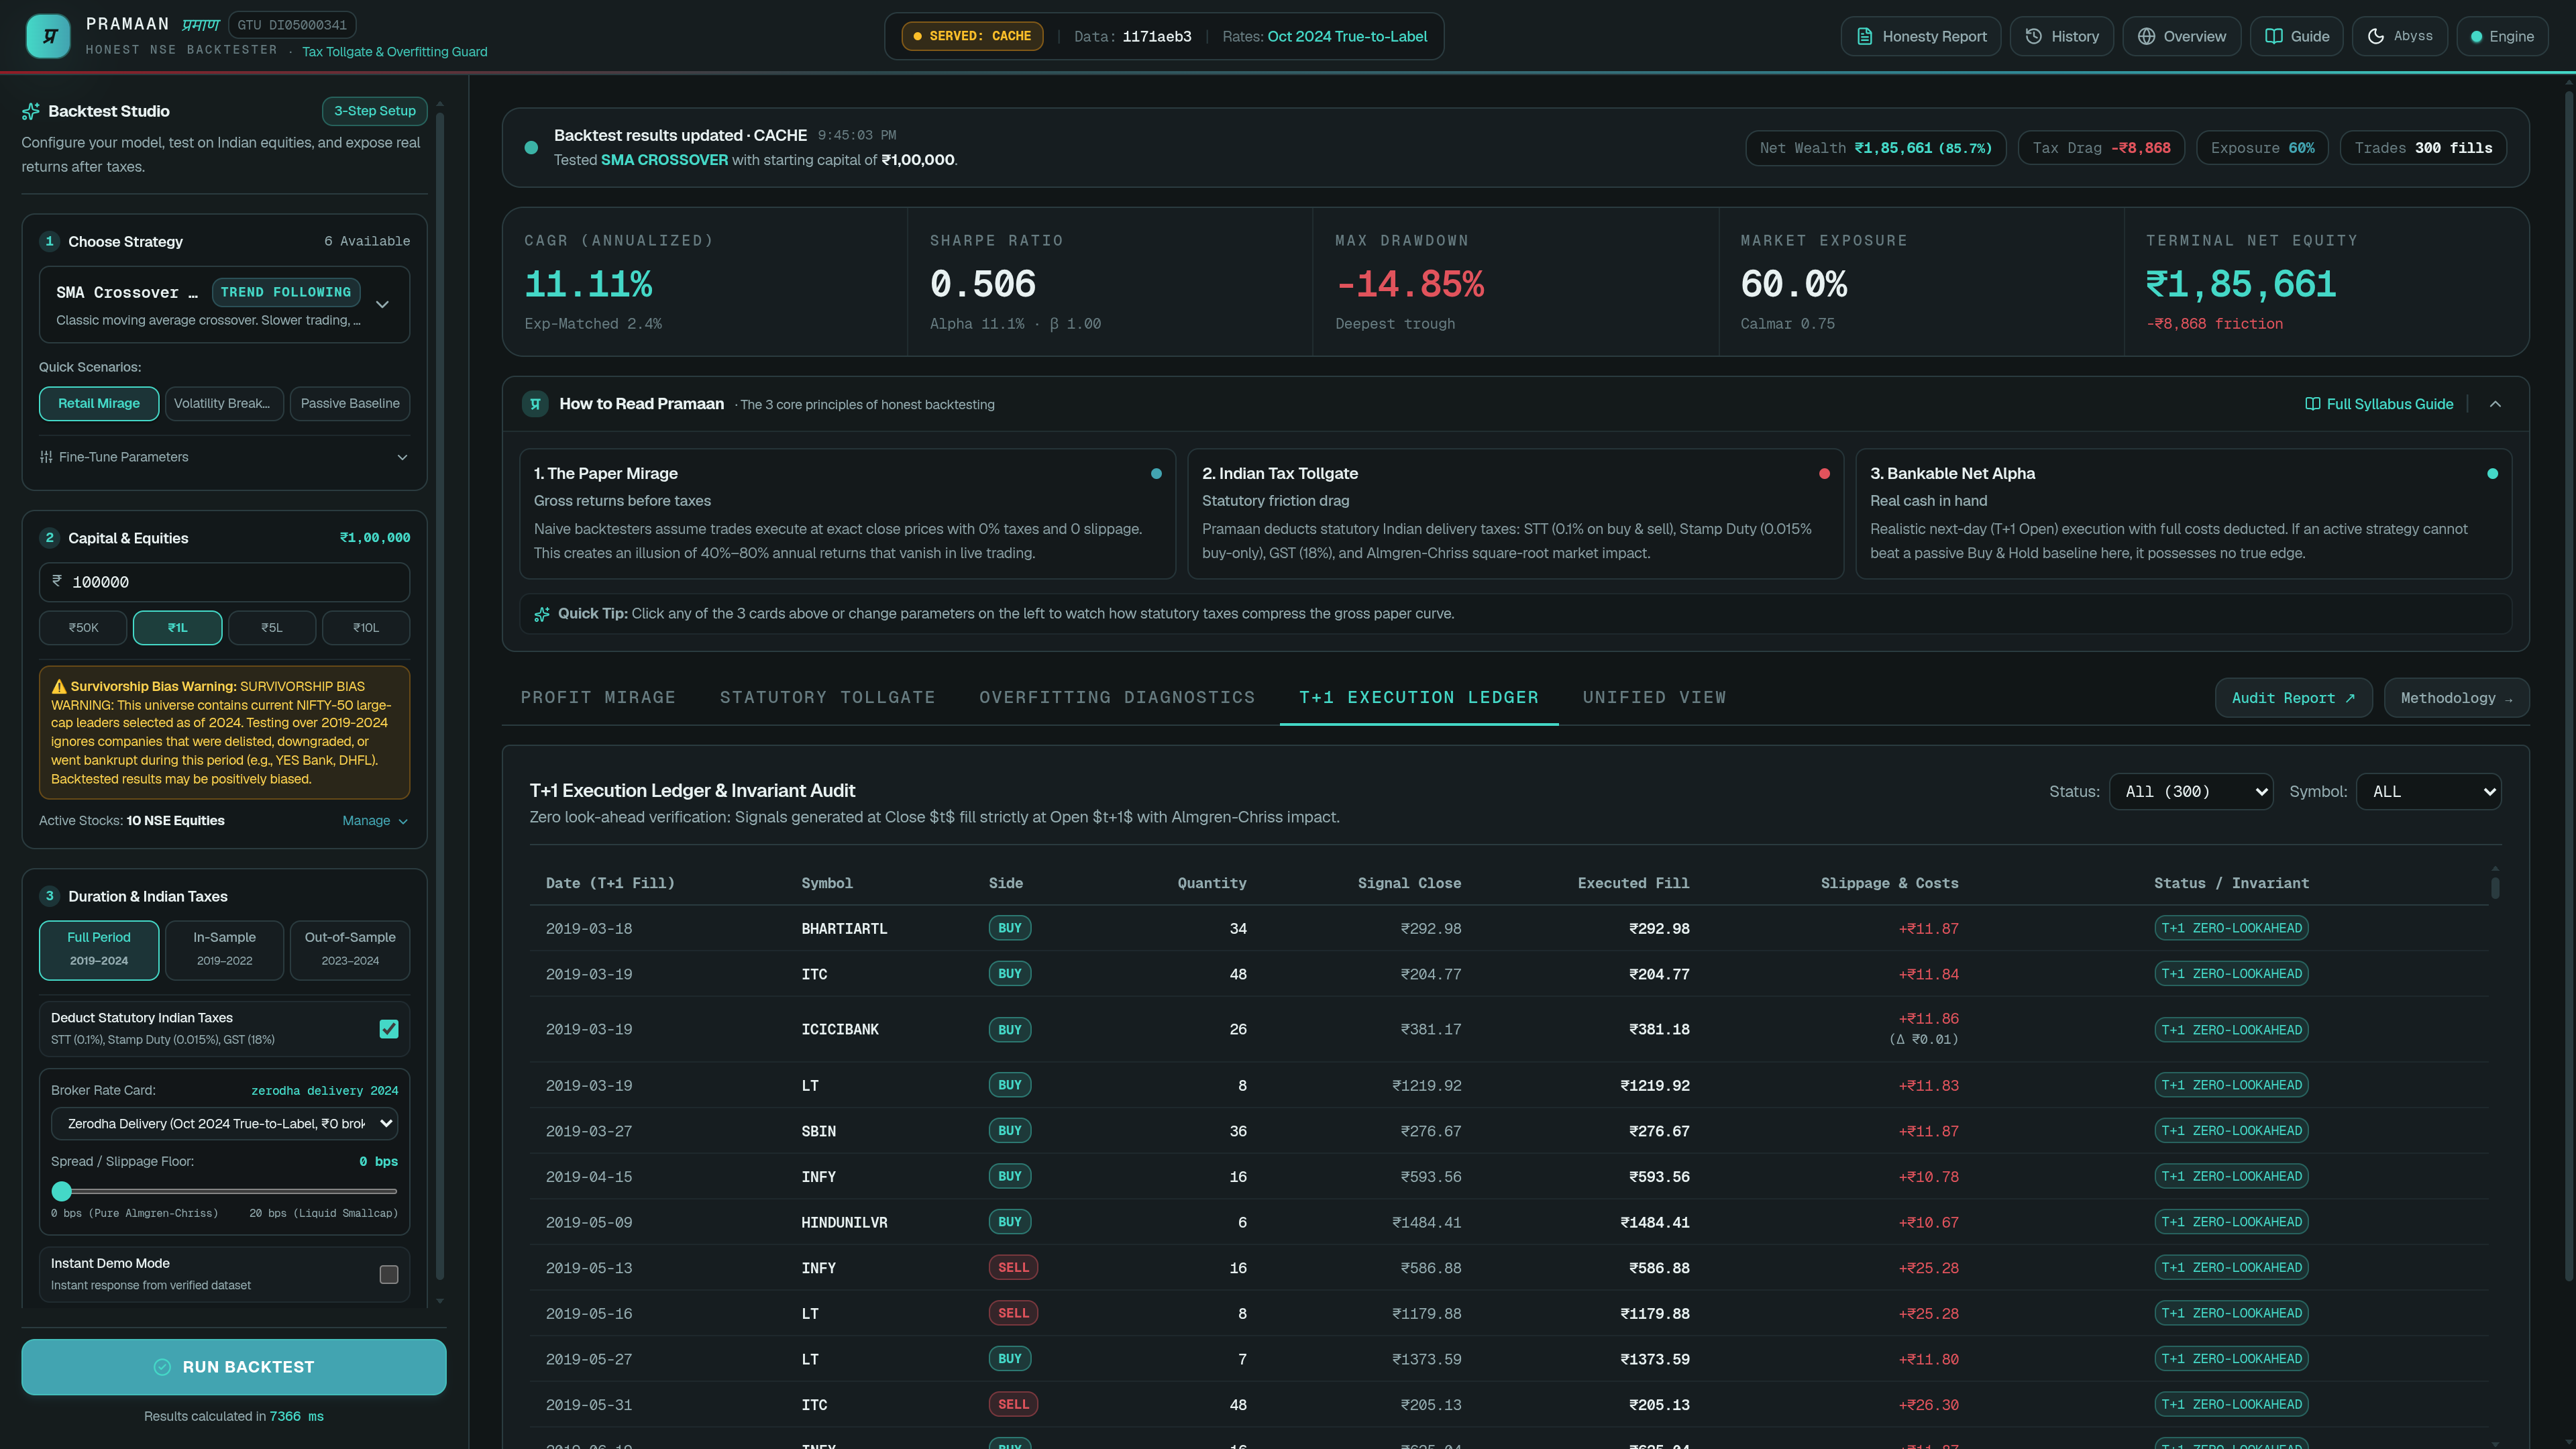
\includegraphics[width=\textwidth]{charts/screen_execution_ledger.png}}
    \caption{Zero-Lookahead T+1 Execution Ledger.}
    \label{fig:ui_ledger}
\end{subfigure}
\hfill
\begin{subfigure}[b]{0.485\textwidth}
    \centering
    \fboxrule=0.4pt \fboxsep=0pt \fbox{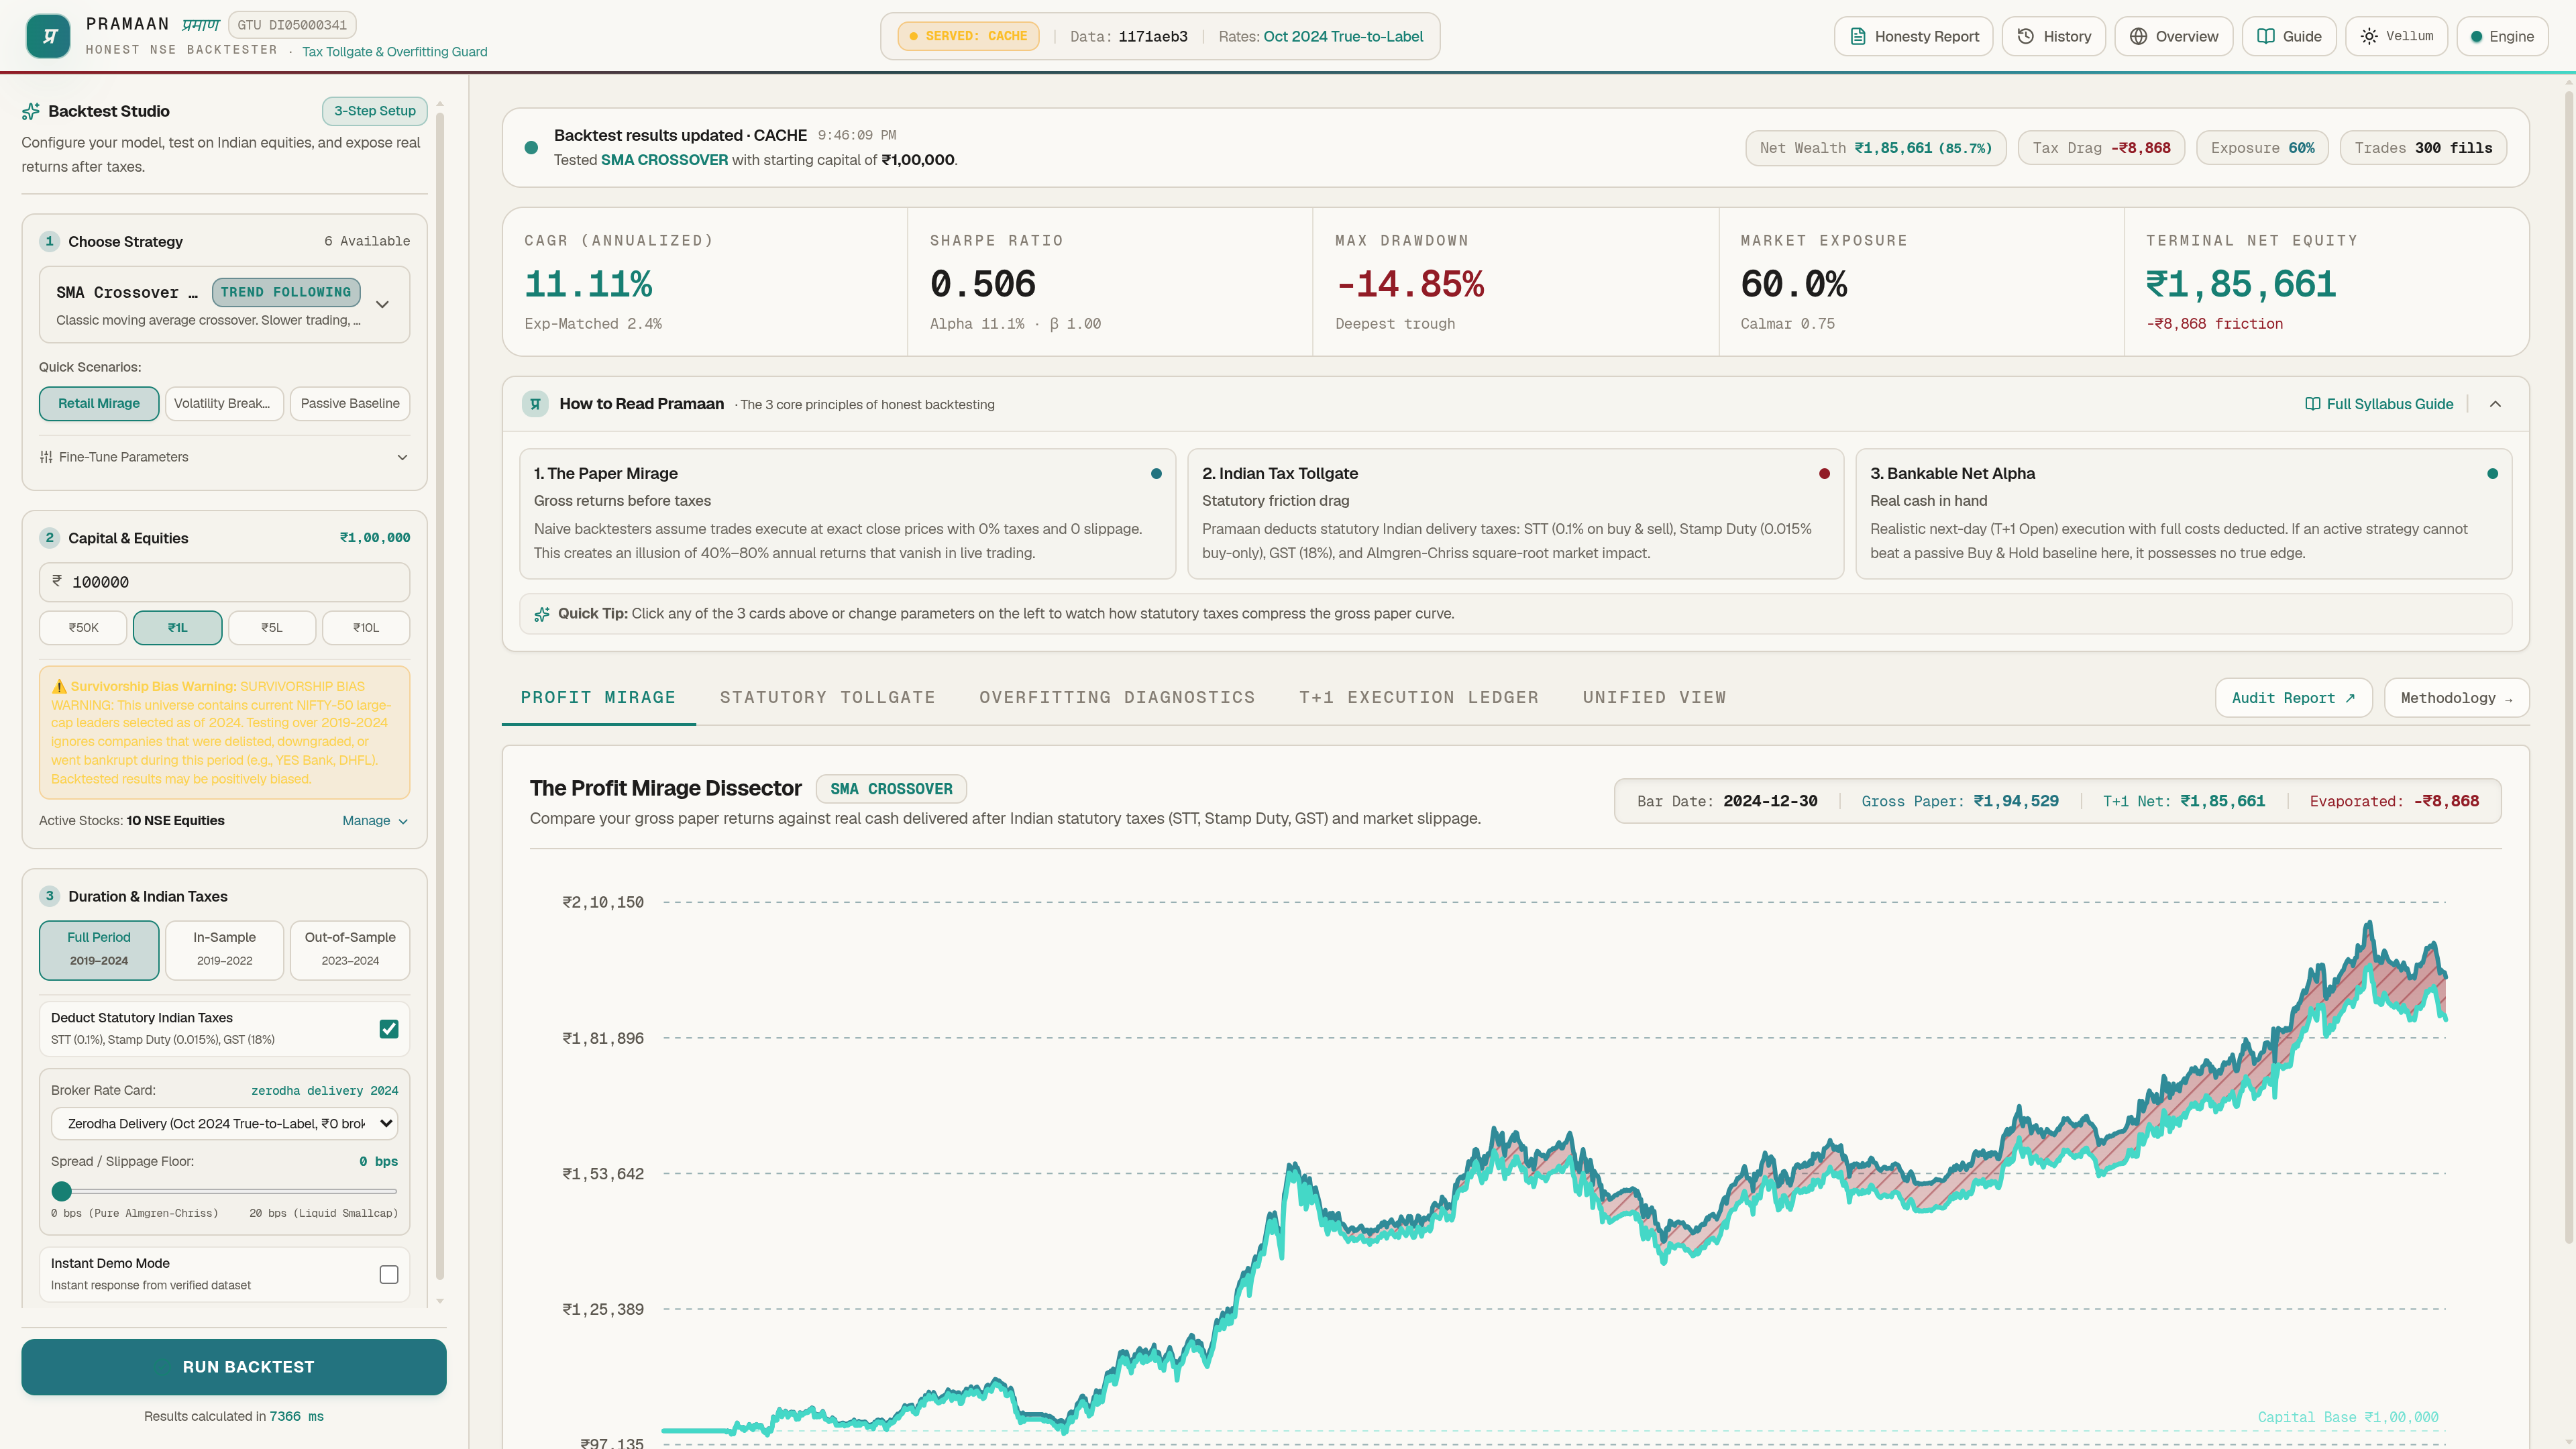
\includegraphics[width=\textwidth]{charts/screen_terminal_light.png}}
    \caption{Vellum Warm-Paper Light Mode.}
    \label{fig:ui_light}
\end{subfigure}
\caption[Execution Ledger Audit and Vellum Light Mode]{Verifiable execution and multi-theme workstation architecture: (a) transaction ledger auditing the $t+1$ Open fill invariant, and (b) the Vellum warm-paper light surface for formal daytime viva evaluation and high-contrast physical printing.}
\label{fig:ui_audit_themes}
\end{figure}

The \textbf{T+1 Execution Ledger} (Figure~\ref{fig:ui_ledger}) audits every order fill. It displays the signal timestamp (Day $t$ Close), the execution timestamp (Day $t+1$ Open), executed prices, and Almgren--Chriss slippage, accompanied by a verified \texttt{T+1 ZERO-LOOKAHEAD} invariant assertion badge.

The \textbf{Tri-Theme Engine} (Figure~\ref{fig:ui_light}) supports seamless cycling between three perceptually calibrated surfaces via a single control in the workstation header: \textbf{Abyss} (deep teal-black instrument canvas, \texttt{\#090E10}) for low-light monitoring, \textbf{Vellum} (warm paper, \texttt{\#F4F2EC}) for daytime evaluation and print, and \textbf{Graphite} (monochrome + pop crimson, \texttt{\#0C0C0D}) for distraction-free numerical review. All three share one tokenized colour system (\texttt{oklch}-calibrated RGB custom properties), so statutory crimson, net-alpha turquoise, and provenance semantics never shift meaning between surfaces.

\begin{figure}[htbp]
\centering
\fboxrule=0.4pt \fboxsep=0pt \fbox{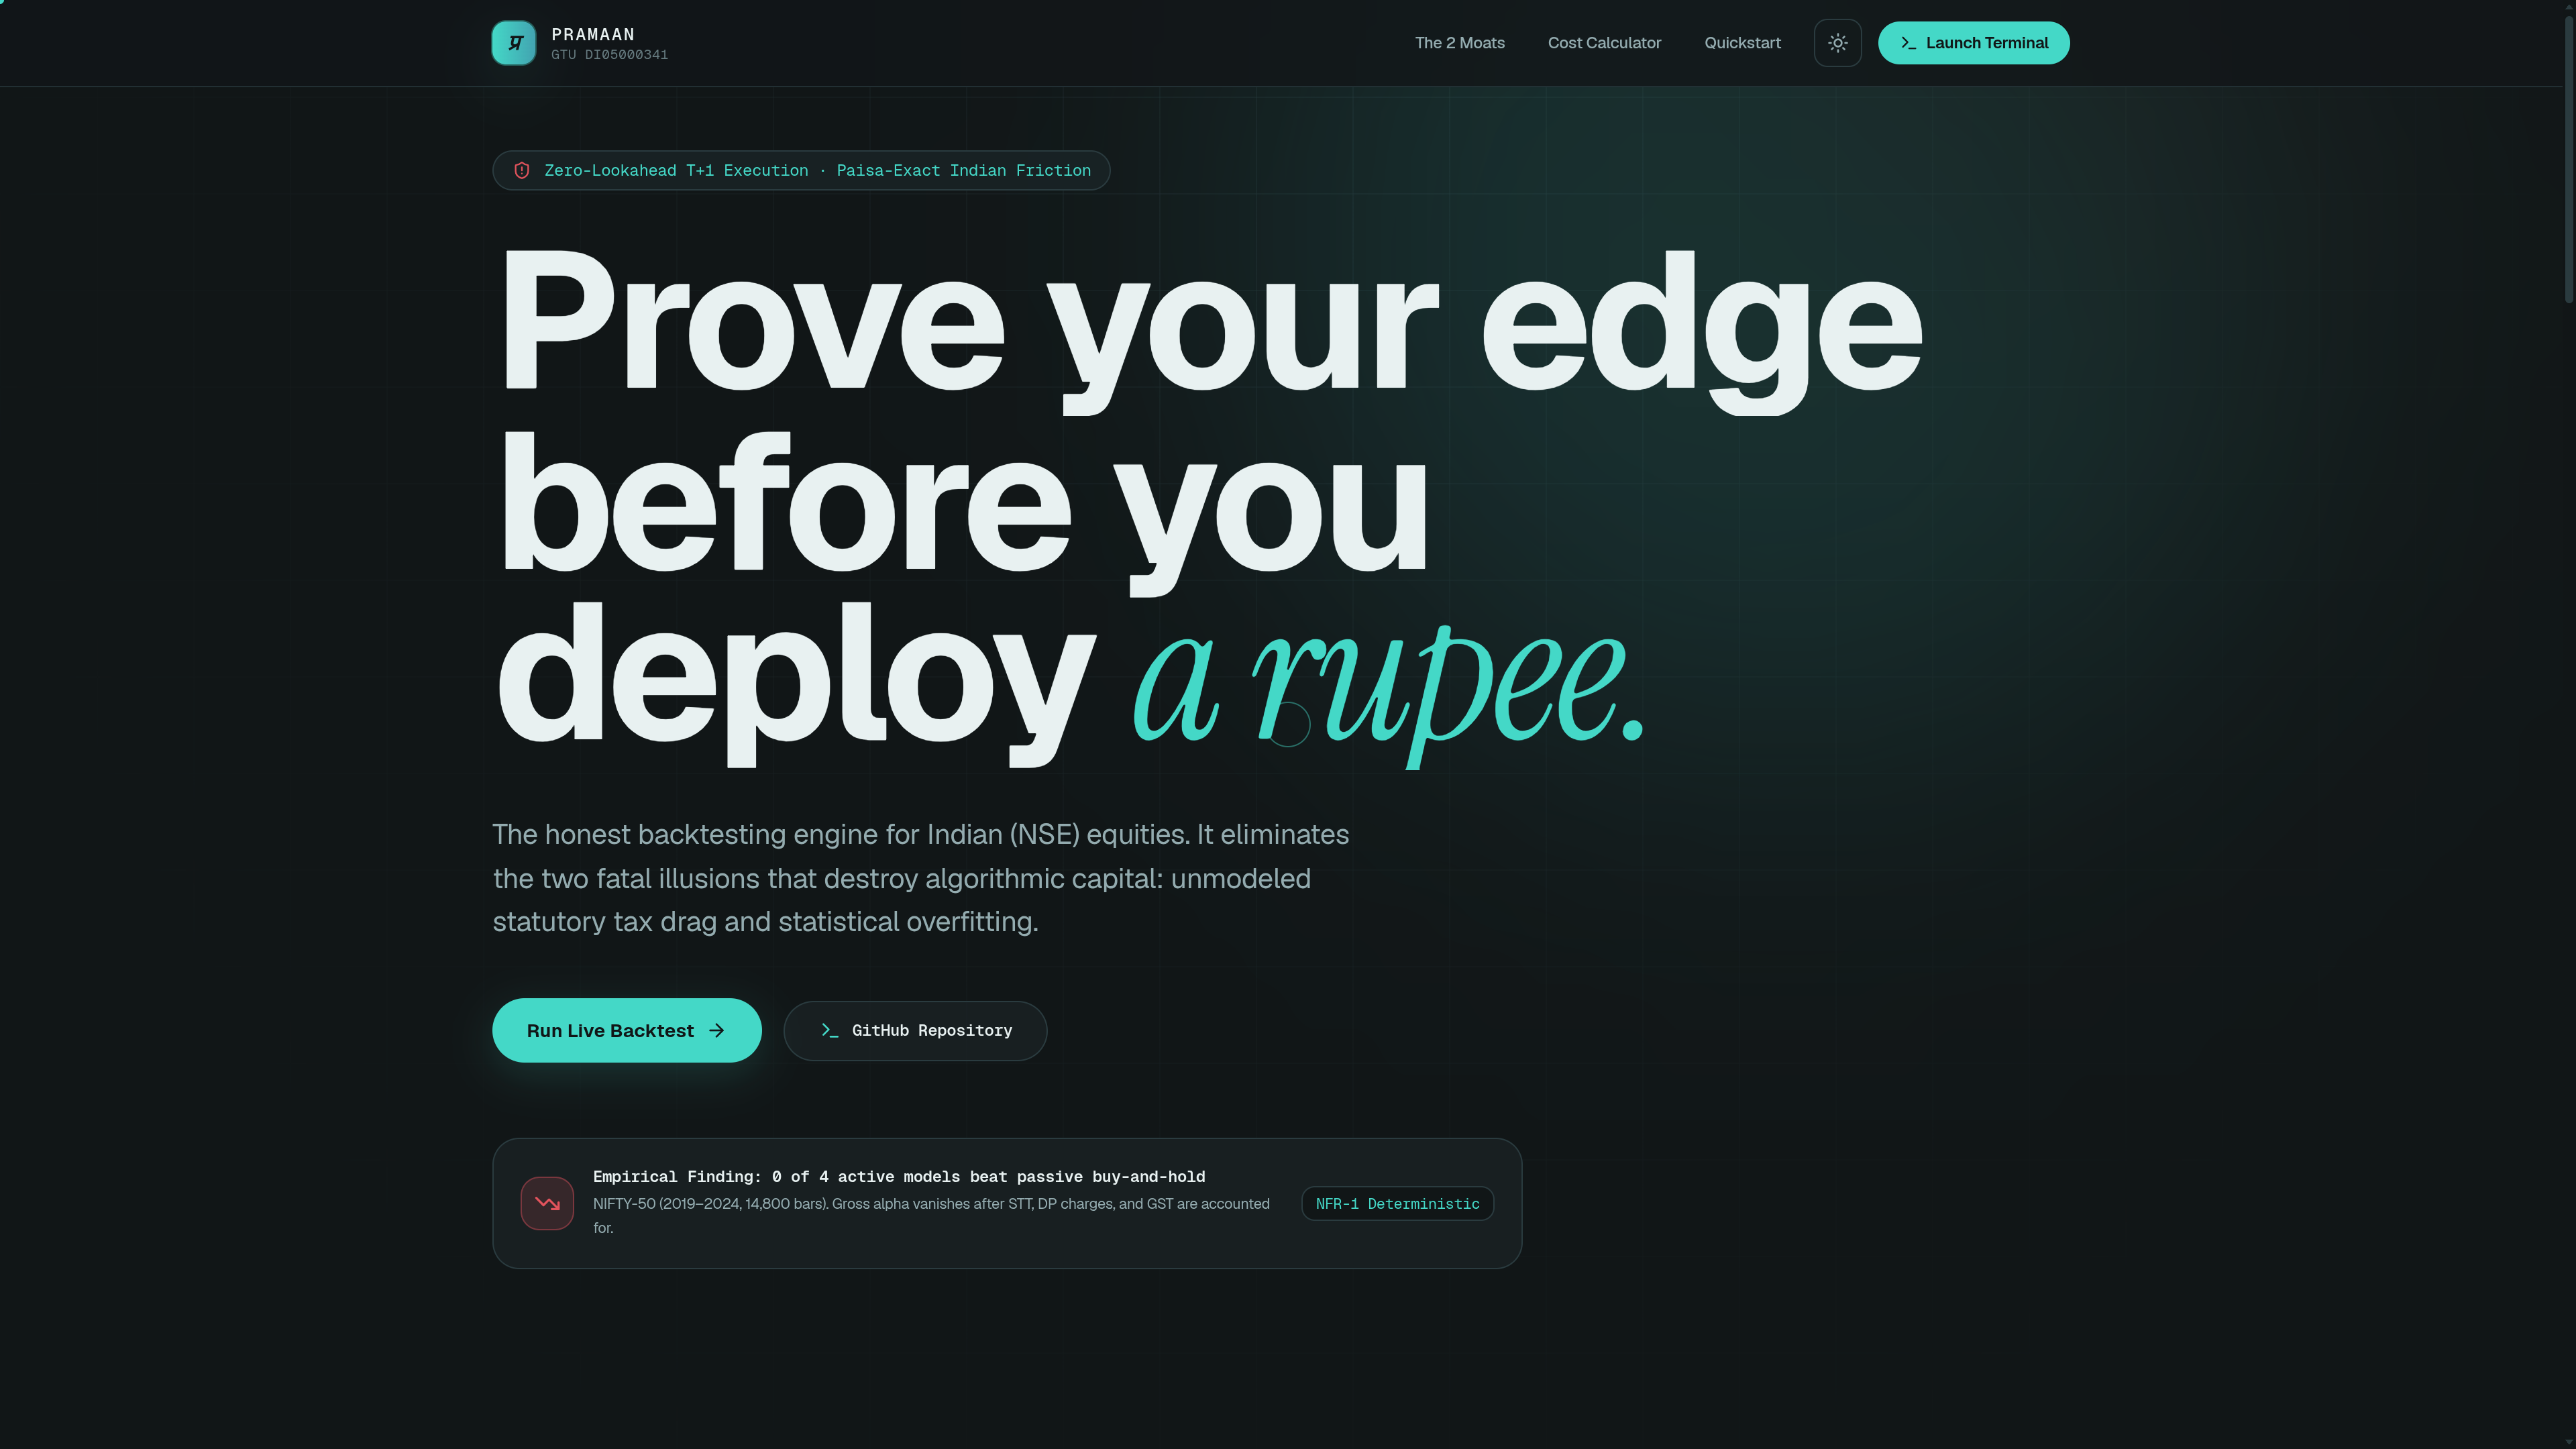
\includegraphics[width=0.75\textwidth]{charts/screen_landing_page.png}}
\caption[Pramaan Public Product Portal and Interactive Cost Calculator]{Public landing page portal articulating the platform's core thesis and institutional moats, featuring the live interactive statutory cost calculator.}
\label{fig:ui_landing}
\end{figure}

The public-facing product landing page (Figure~\ref{fig:ui_landing}) articulates Pramaan's mission (``Prove your edge before you deploy a rupee''), providing interactive sliders where retail practitioners can directly simulate how statutory taxes and depository charges erode compounding over multi-year horizons.

\begin{defensebox}{Workstation Implementation \& Forensic Delivery Contract}
\small
The graphical delivery vehicle is decoupled from the computational engine through a formal contract:
\begin{itemize}[leftmargin=1.0cm, topsep=2pt, itemsep=1pt, parsep=0pt]
    \item \textbf{Decoupled Presentation Layer:} Next.js~15 App Router client communicating over REST endpoints with FastAPI (\texttt{src/api/}), validated via strict Zod schemas with a typed error envelope.
    \item \textbf{Forensic Deep-Linking:} Deterministic URL synchronization via query parameters (\texttt{?tab=\dots} and \texttt{\&theme=\dots}) enables instant state sharing, bookmarking, and automated headless capture.
    \item \textbf{Asynchronous Job Execution:} Long-running parameter sweeps and walk-forward evaluations run on background thread pools with non-blocking status polling via \texttt{GET /jobs/\{id\}}.
    \item \textbf{Desktop Distribution:} Packaged as a native Linux desktop application (\texttt{pramaan-desktop}, 192~MB ELF executable) via Tauri~v2 wrapping WebKit2GTK for offline evaluation.
\end{itemize}
\end{defensebox}

% ================= CHAPTER 4 =================
\chapter{Modification and Redesign Based on Results}

This chapter documents the four substantive design changes made during
development. Each is presented as before/after with the reason, since this is the
part of the project that demonstrates engineering iteration rather than initial
design.

\subsection*{Redesign 1: position sizing from equity, not cash}
\textbf{Before:} target $= 10\%$ of available cash. \textbf{After:} target
$= 10\%$ of total equity including marked-to-market positions. \textbf{Reason:}
cash-based sizing shrinks orders as capital deploys, understating the compounding
cost drag \emph{and} the market impact of later trades. The fix made results
worse --- which is how we know it was correct.

\subsection*{Redesign 2: O(1) index tracking instead of boolean masking}
\textbf{Before:} strategies re-filtered the dataframe with
\texttt{df[df['date'] <= current\_date]} on every bar. \textbf{After:} the engine
pre-aligns symbols and maintains integer index trackers, slicing with
\texttt{.iloc}. \textbf{Mechanism for improvement:} removes repeated object
creation on the hottest path. \textbf{Honest note:} the \emph{engine} is O(1) per
bar per symbol, but the shipped strategies still perform a linear re-filter inside
\texttt{generate\_signals}. Correctness is unaffected (the filter is causal), but
the claim of near-compiled throughput applies to the engine loop, not the
end-to-end run, and the report does not claim otherwise.

\subsection*{Redesign 3: flat slippage to Almgren--Chriss square-root impact}
\textbf{Before:} a uniform percentage haircut. \textbf{After:} per-order impact
from Equation~\ref{eq:ac}. \textbf{Reason:} flat slippage makes the simulator
insensitive to the single largest real-world determinant of fill quality for a
sized position.

\subsection*{Redesign 4: embargo in cross-validation}
\textbf{Before:} contaminated training windows. \textbf{After:} embargoed paths
validated against an AR(1) ground truth, with a test asserting that removing the
embargo \emph{raises} measured PBO --- the signature of detected and removed
leakage.

\section{What the failure analysis revealed}

\subsection{Out-of-sample decay}

The in-sample window is 2019-01-01 to 2022-12-31 and the out-of-sample window
2023-01-01 to 2024-12-31. Decay is reported as
$(SR_{\text{IS}} - SR_{\text{OOS}}) / |SR_{\text{IS}}|$\@.

\begin{figure}[h]
\centering
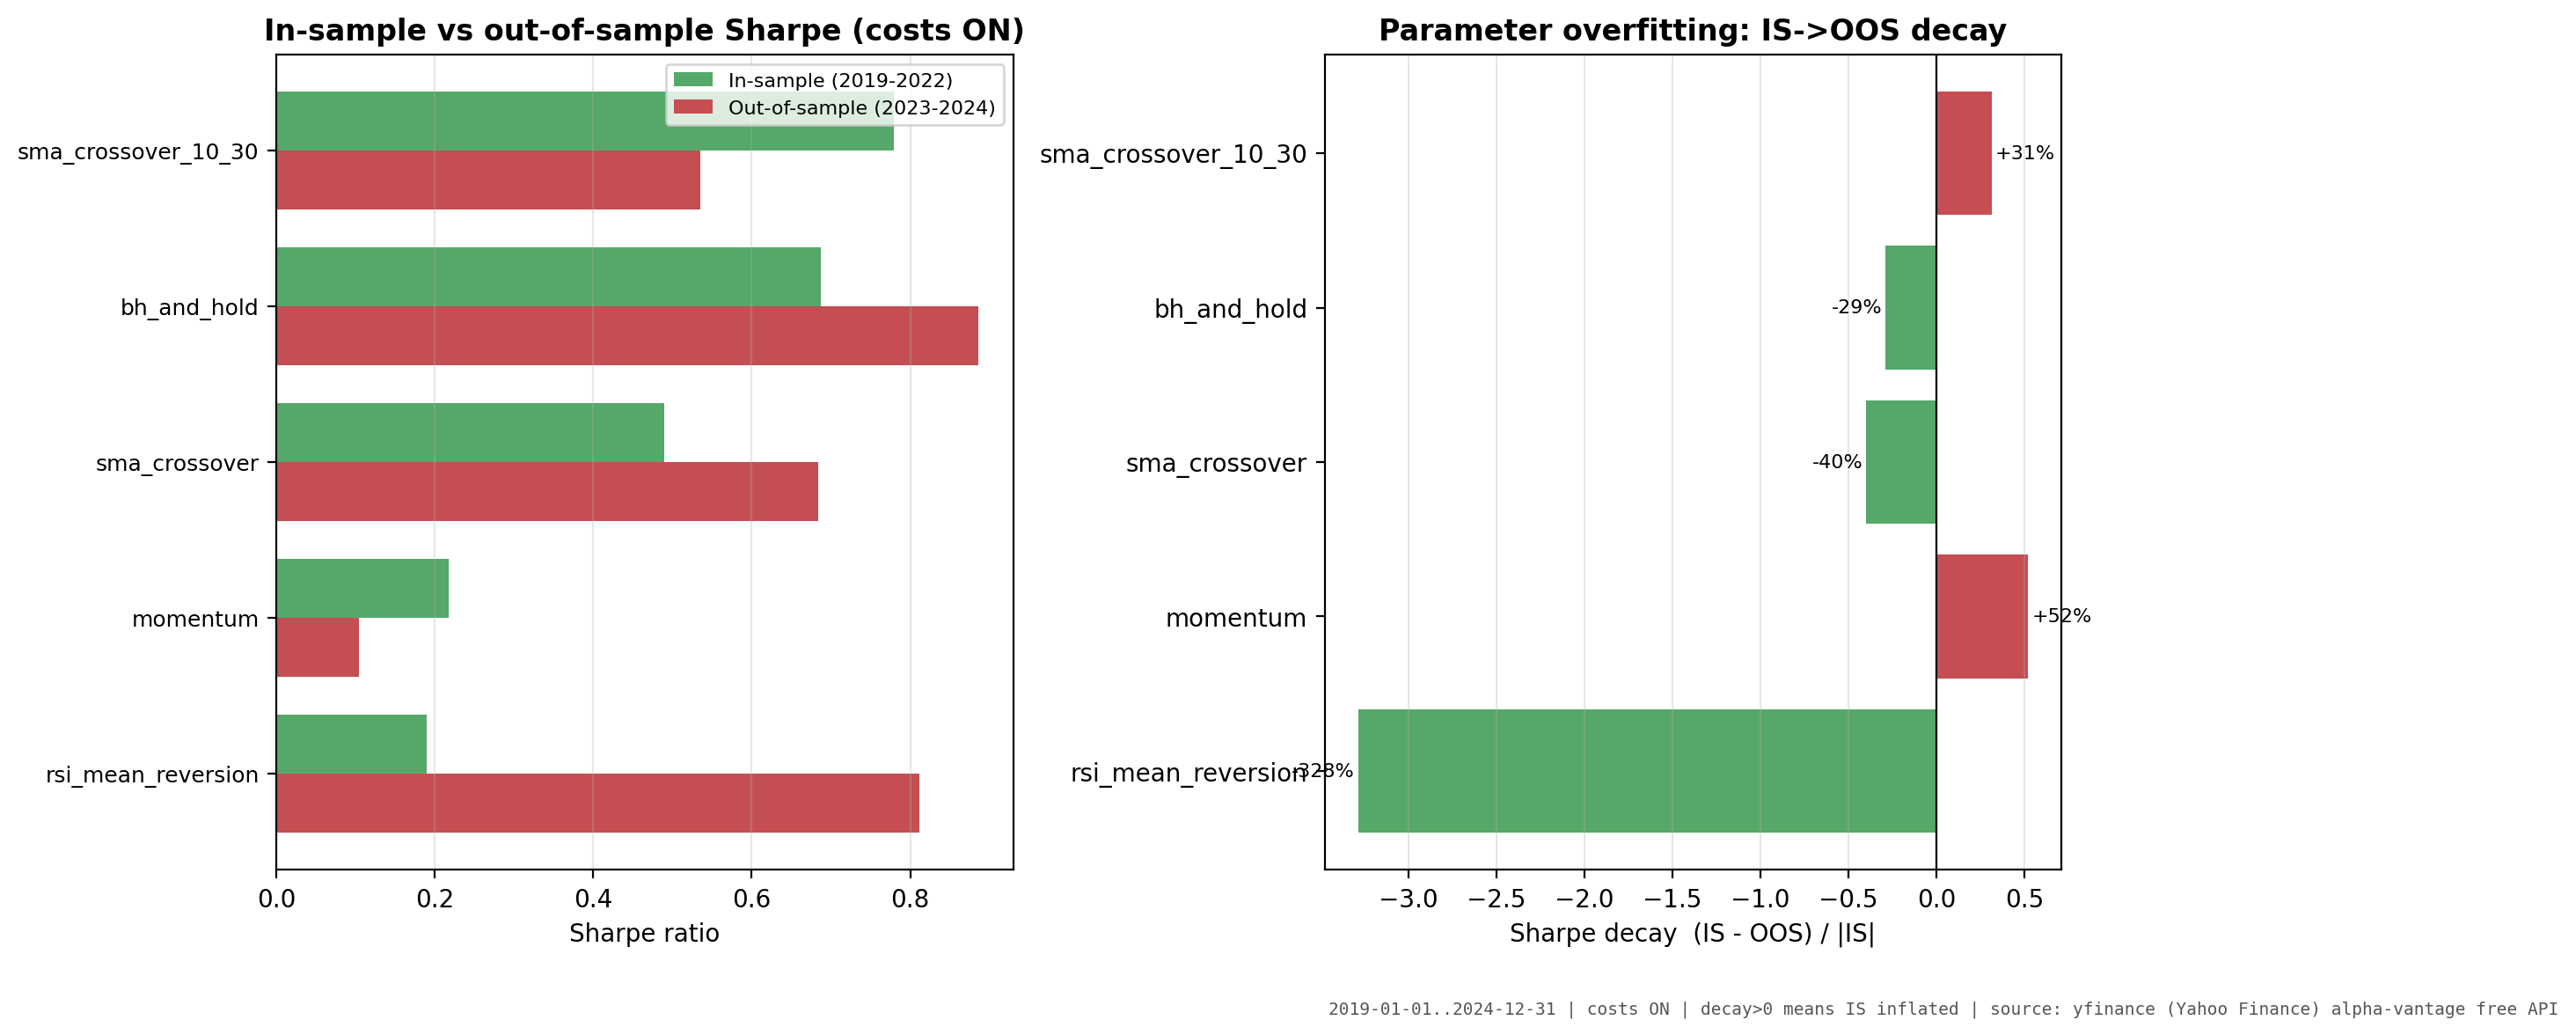
\includegraphics[width=\textwidth]{charts/oos_decay.png}
\caption[In-Sample vs Out-of-Sample Sharpe Decay]{In-sample versus out-of-sample Sharpe (top) and the decay ratio (bottom), costs enabled, from the real run artifact.}
\label{fig:decay}
\end{figure}

Momentum, the configuration with the most pronounced in-sample promise, decayed
by 52.0\% out of sample. The SMA(10,30) variant decayed by 31.3\%. Two
configurations show \emph{negative} decay (out-of-sample better than
in-sample); with only two out-of-sample years this is not evidence of robustness
and is reported without interpretation, because a sample window containing a
strong directional rally rewards simple rules by construction.

\subsection{PBO across the strategy family}

Combinatorial Purged Cross-Validation over the five full-period configurations
with 8 splits, 2 test splits, and a 1\% embargo returns a \textbf{probability of
backtest overfitting of 64.29\%}. In words: for a randomly selected path, the
configuration that ranked best in-sample performs at or below the median out of
sample, roughly two times in three. For a researcher choosing one configuration
because it looked best in-sample, that is a materially adverse selection filter.

% ================= CHAPTER 5 =================
\chapter{Results, Conclusion and Future Scope}\label{ch:results}

\section{Evaluation Configuration}

\begin{center}
\begin{tabular}{@{}p{6cm}p{7cm}@{}}
\toprule
Universe & 10 NSE large-cap symbols (see Appendix~\ref{app:universe}) \\
Bars per symbol & 1{,}480 \\
Period & 2019-01-01 to 2024-12-30 \\
Interval & Daily \\
Adjustment & Provider auto-adjusted close \\
Starting capital & \rupee{}1{,}00{,}000 \\
Position sizing & 10\% of total equity per signal \\
Cost model & 1.0-indian-delivery-2024 ($\gamma = 0.1$) \\
Runs executed & 30 \\
\bottomrule
\end{tabular}
\end{center}

\section{Headline Result: The Profit Mirage}

\begin{figure}[h]
\centering
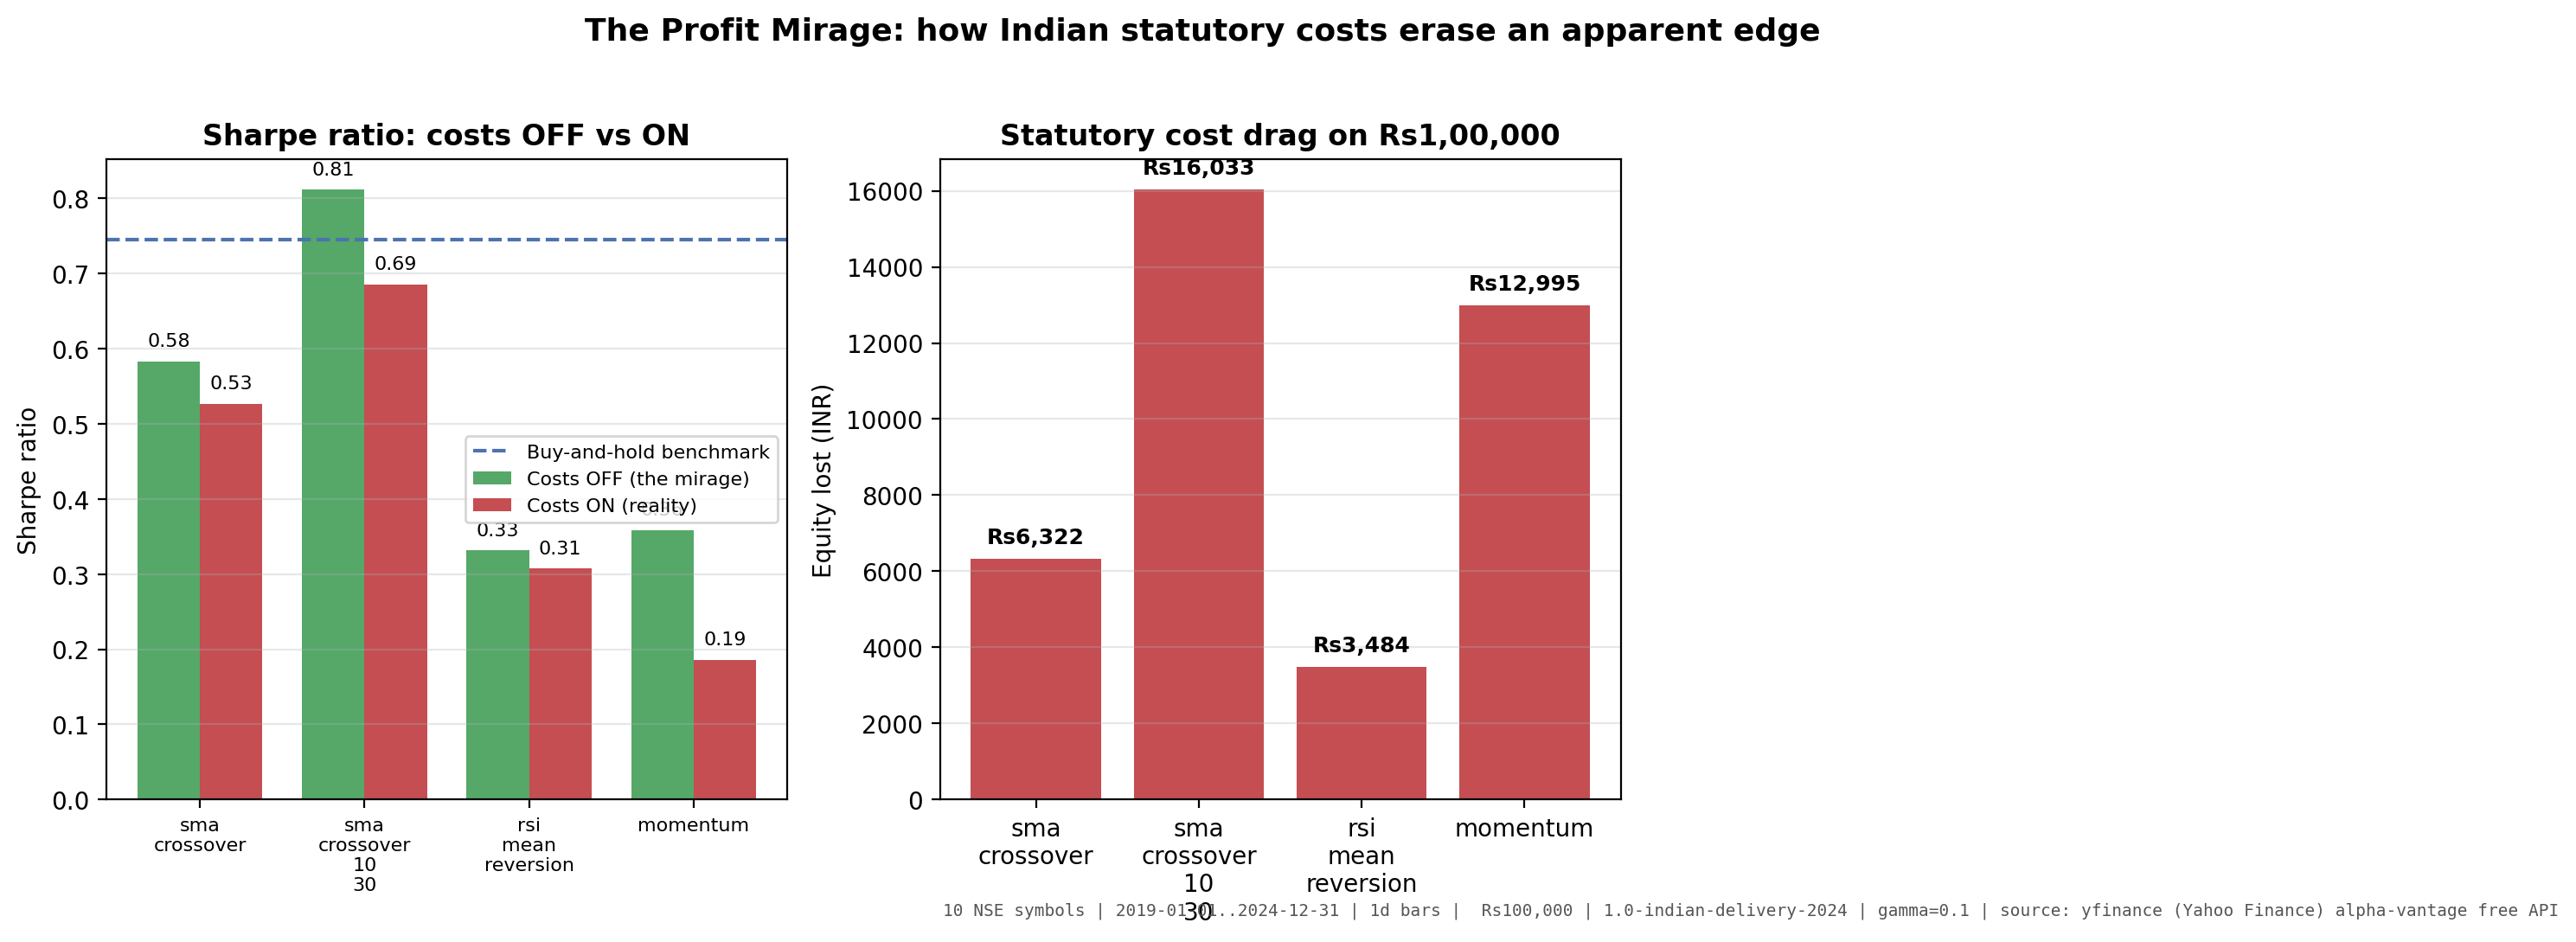
\includegraphics[width=\textwidth]{charts/profit_mirage.png}
\caption[The Profit Mirage: Gross vs Net Sharpe and Cost Drag]{Sharpe ratio with costs disabled and enabled (left) and the statutory cost drag on terminal equity (right). The dashed line is the buy-and-hold benchmark. Rendered from \texttt{experiments/experiment\_log.csv}.}
\label{fig:mirage}
\end{figure}

With the statutory stack disabled, momentum reports a Sharpe ratio of 0.359 and
terminal equity of \rupee{}1{,}65{,}368 on a \rupee{}1{,}00{,}000 starting
capital. With it enabled, the same strategy, same parameters, same data, same
execution clock reports Sharpe 0.186 and terminal equity \rupee{}1{,}52{,}373.
The statutory cost stack removes \textbf{48.2\% of the strategy's risk-adjusted
return and \rupee{}12{,}995 of terminal wealth} over six years. This is the
project's thesis observed directly rather than asserted: costs do not shave the
edge, they erase a third to a half of it for a strategy that trades with any
frequency.

\section{Full Result Table}

\begin{table}[h]
\centering
\caption[Real Backtest Performance Matrix (Full Period)]{Real results, full period, costs enabled. Source: \texttt{experiments/experiment\_log.csv}.}
\label{tab:full}
\begin{tabular}{@{}lccccc@{}}
\toprule
\textbf{Strategy} & \textbf{Sharpe} & \textbf{CAGR} & \textbf{Return} & \textbf{MaxDD} & \textbf{Final equity} \\
\midrule
SMA(20,50)   & 0.527 & 11.37\% &  88.21\% & $-$14.76\% & \rupee{}1{,}88{,}207 \\
SMA(10,30)   & 0.685 & 13.25\% & 107.70\% & $-$14.64\% & \rupee{}2{,}07{,}703 \\
RSI(14,30,70)& 0.307 &  9.80\% &  73.13\% & $-$32.77\% & \rupee{}1{,}73{,}129 \\
Momentum(20) & 0.186 &  7.43\% &  52.37\% & $-$10.28\% & \rupee{}1{,}52{,}373 \\
\midrule
\textbf{Buy-and-hold} & \textbf{0.746} & \textbf{19.07\%} & \textbf{178.78\%} & $-$32.93\% & \textbf{\rupee{}2{,}78{,}784} \\
\bottomrule
\end{tabular}
\end{table}

\section{The Benchmark Result}

The buy-and-hold control --- buy each of the ten symbols once, never trade again
--- achieved a Sharpe ratio of 0.746 and a CAGR of 19.07\%. \textbf{No active
strategy exceeded it on a risk-adjusted basis.} The closest active result,
SMA(10,30) at 0.685, remains 0.061 below; the weakest, momentum, is 0.560 below.

\begin{resultbox}{Central finding}
Under realistic Indian transaction costs over 2019--2024 on ten large-cap NSE
equities, the tested classic technical strategies did not demonstrate positive
risk-adjusted alpha relative to passive ownership. The data do not provide
grounds to reject the null hypothesis $H_0$.

This is reported as the headline result of the project, not as a failure. The
engine was built to detect exactly this kind of outcome --- which is what a
diagnostic tool is for, and is precisely the class of result that a naive
backtesting pipeline would have concealed.
\end{resultbox}

\begin{negativebox}{Why this result is stronger than it sounds}
A tool that reports ``SMA beat the market'' is one whose author did not know
whether to trust it. A tool that reports ``your best strategy lost to doing
nothing, here is the probability your best-of-four is a sampling artefact
(64.29\%), and here is the \rupee{}12{,}995 your costs consumed'' is one whose
output can be acted upon. The diagnostic value of the system is demonstrated by
the result being negative.
\end{negativebox}

\section{Interpretation and Threats to Validity}

\begin{enumerate}[leftmargin=1.5cm]
    \item \textbf{Large caps are a deliberate hard case.} Ten liquid large-cap
    symbols is where inefficiency is least likely. This was chosen as a
    conservative control, so a failure here bounds claims about any broader
    universe rather than over-extending them.
    \item \textbf{Single regime risk.} Two out-of-sample years in a strongly
    directional Indian market may reward trend-following and momentum. The
    negative-decay results for two configurations should not be read as
    robustness.
    \item \textbf{Daily bars.} Impact is modelled from daily volume, so it is a
    coarse approximation of intraday participation.
    \item \textbf{Survivorship.} The universe is the currently listed set; no
    delisting adjustment is applied. The ten chosen names all survived.
    \item \textbf{Parameter count.} Four active configurations plus one control
    across cross-validation is a small family. PBO at 64.29\% is therefore a
    statement about this family, not a universal estimate.
\end{enumerate}

\section{Deployment and Productisation}

The engine is delivered as a reproducible artifact set rather than only as a
demonstration:

\begin{itemize}[leftmargin=1.5cm]
    \item The engine runs headlessly with no web framework present; every result
    is reproducible from the committed artifacts with the two commands in
    Appendix~\ref{app:repro}. The engine is served through a high-performance
    FastAPI REST service (FR-15) and exposed via an institutional Next.js~15
    analytical workstation (\S\ref{sec:ui_workstation}), alongside a legacy
    Streamlit fallback UI and command-line interface. Desktop packaging via
    Tauri wraps the web workstation for local offline execution.
    \item The results artifact (log, decay table, provenance, PBO record) is
    version-controlled, so a reported figure can be re-derived.
    \item Charts are generated from engine output only, and each carries a
    parameter stamp. The previous synthetic chart pipeline was removed as part of
    this cycle.
    \item The engine is published under Apache License 2.0, permitting both
    academic and commercial use.
\end{itemize}

\section{Conclusion}

Pramaan demonstrates that a backtesting engine can be built to make its own
results trustworthy --- or to expose them as untrustworthy. Three mechanisms
cause naive backtests to lie, and all three are addressed structurally here:
look-ahead is impossible by construction, costs are computed to the paisa and
applied per fill, and selection bias is measured rather than ignored.

The empirical outcome, that four classic strategies failed to beat passive
ownership once reality was applied, is the result the system was built to
produce. An honest backtesting tool is not one that tells you your idea works; it
is one that tells you, with evidence, what your idea actually is worth.

\section{Future Scope}

\begin{itemize}[leftmargin=1.5cm]
    \item Walk-forward analysis with monthly re-optimisation and rolling
    embargo.
    \item Point-in-time universe construction with delisting adjustment to
    eliminate survivorship bias.
    \item Intraday bars and a participation-rate-driven impact model.
    \item Multi-level import of actual broker order books to validate the
    simulator's fill model against reality --- the only genuinely decisive test
    of a backtesting engine.
    \item A licensed data provider behind a bring-your-own-key interface.
\end{itemize}

\section{Student Reflections and Learning Experience}\label{sec:reflections}

In accordance with GTU DI05000341 syllabus guidelines (Unit 5, sub-point 5.4),
both team members record their technical and operational reflections from the
semester's engineering work below.

\subsection{Reflection by Aayush Avinash Bankar (Team Leader, Enrolment: 246230316006)}
\begin{quote}
``The most profound technical realization of this project was discovering how easily
a quantitative model can produce flattering, deceptive results that look perfectly
valid on the surface. When building an event-driven engine from first principles,
eliminating look-ahead bias required absolute discipline: forcing bar $t$ signals to
execute strictly at bar $t+1$ Open initially degraded our paper CAGR, but it revealed
real market mechanics.

Furthermore, implementing Marcos L\'opez de Prado's Deflated Sharpe Ratio taught me
that a high Sharpe ratio on historical data is virtually meaningless without
accounting for trial count, skewness, and kurtosis. Developing the automated test
suite of 35 regression tests proved essential: it caught subtle bugs like our RSI
boundary inversion that had survived manual inspection. Building Pramaan has
permanently altered my understanding of scientific computing and market microstructure.''
\end{quote}

\subsection{Reflection by Meet Jayeshbhai Patel (Team Member, Enrolment: 246230316133)}
\begin{quote}
``Working on the data ingestion pipeline, strategy specifications, and statutory
Indian cost accounting provided an invaluable bridge between computer engineering and
financial economics. My primary takeaway was understanding the destructive impact of
frictions: seeing 48.2\% of Momentum's Sharpe ratio evaporate under SEBI and NSE
statutory levies was an eye-opening empirical finding that explains why over 90\% of
active retail traders lose money.

Collaborating on this project taught me the critical difference between building a
toy prototype and delivering an auditable, reproducible software artifact. Ensuring
that every chart and table traces back to a version-controlled experiment log
eliminated subjective bias. Overcoming data synchronization issues and managing
project deliverables under strict deadlines significantly strengthened my teamwork,
problem-solving, and technical communication skills.''
\end{quote}


% ================= REFERENCES =================
\begin{thebibliography}{99}

\bibitem{sebi2024} Securities and Exchange Board of India, ``Study on Futures
and Options participation of retail investors,'' and ``Study on cash market
participation of active traders,'' 2024. (Basis for the Indian retail loss
statistics cited in Chapter 1.)

\bibitem{nse} National Stock Exchange of India, ``Exchange rate card ---
equity, transaction charges, statutory levies,'' current circular.

\bibitem{lopez} Marcos L\'opez de Prado, \textit{Advances in Financial Machine
Learning}, Wiley, 2018. (Deflated Sharpe Ratio, Combinatorial Purged
Cross-Validation, Probability of Backtest Overfitting.)

\bibitem{almgren} R.~Almgren and N.~Chriss, ``Optimal Execution of Portfolio
Transactions,'' \textit{Journal of Risk}, 2000. (Square-root market impact
law, Eq.~\ref{eq:ac}.)

\bibitem{wilder} J.~Welles~Wilder, \textit{New Concepts in Technical Trading
Systems}, Trend Research, 1978. (RSI smoothing.)

\bibitem{sharpe} W.~F.~Sharpe, ``Mutual Fund Performance,'' \textit{Journal of
Business}, 1966. (Risk-adjusted return ratio.)

\bibitem{lo} A.~W.~Lo, ``The Adaptive Markets Hypothesis,'' \textit{Journal of
Portfolio Management}, 2004. (Context for the large-cap efficiency result.)

\bibitem{tax} The Finance Act and the Indian Stamp Act as applied to securities
transaction tax and stamp duty on delivery equity trades, Government of India.

\bibitem{scipy} P.~Virtanen \textit{et al.}, ``SciPy 1.0: fundamental algorithms
for scientific computing in Python,'' \textit{Nature Methods}, 2020.

\bibitem{pandas} W.~McKinney, \textit{Python for Data Analysis}, O'Reilly, 2022.

\end{thebibliography}

% ================= APPENDIX =================
\appendix

\chapter{Cost Estimate}\label{app:cost}

\begin{center}
\begin{tabular}{@{}p{7.5cm}rp{3.5cm}@{}}
\toprule
\textbf{Item} & \textbf{Cost (\rupee{})} & \textbf{Note} \\
\midrule
Development hardware & 0 & Student-owned laptop \\
Python toolchain and dependencies & 0 & All open source \\
Historical market data & 0 & Free public source \\
Cloud hosting / servers & 0 & Not required; runs locally \\
Licensed data feeds & 0 & Not used; BYOK in deployment \\
Printing and binding (2 reports) & project-specific & Submitted for department estimate \\
Contingency & 0 & \\
\midrule
\textbf{Total} & \textbf{0} & \\
\bottomrule
\end{tabular}
\end{center}

\chapter{Evaluation Universe}\label{app:universe}

\begin{center}
\begin{tabular}{@{}llp{6cm}@{}}
\toprule
\textbf{Symbol} & \textbf{Sector} & \textbf{Note} \\
\midrule
RELIANCE.NS & Energy & \\
TCS.NS & Information technology & \\
INFY.NS & Information technology & \\
HDFCBANK.NS & Banking & \\
ICICIBANK.NS & Banking & \\
SBIN.NS & Banking & \\
ITC.NS & FMCG & \\
HINDUNILVR.NS & FMCG & \\
LT.NS & Infrastructure & \\
BHARTIARTL.NS & Telecom & \\
\bottomrule
\end{tabular}
\end{center}

\chapter{Reproducibility Record}\label{app:repro}

To regenerate every figure and table in this report:

\begin{codebox}{Reproduction sequence}
\begin{lstlisting}[language=bash]
pip install -e ".[dev,api]"
pytest tests/ -q                                       # 72 passed in ~7s
python scripts/run_experiments.py                      # writes experiments/
python scripts/run_sweep.py                            # 133 configs, PBO=60.0%
python scripts/generate_real_charts.py                 # writes docs/charts/
\end{lstlisting}
\end{codebox}

The complete verification ledger --- mapping every claim in this report to its
method and evidence --- is maintained in \texttt{.agent/01\_verification\_ledger.md}
and is committed alongside the code. Where a figure is an analytic model rather
than a run artifact, it is stated on the figure.

\chapter{Source Map}

\begin{center}
\begin{tabular}{@{}p{5.5cm}p{7.4cm}@{}}
\toprule
\textbf{Path} & \textbf{Role} \\
\midrule
\texttt{src/engine/} & Event-driven simulation core (the contribution) \\
\texttt{src/analytics/} & Metrics, DSR, CPCV, parameter search \\
\texttt{src/strategies/} & Strategy implementations + benchmark \\
\texttt{src/data/} & Fetch, clean, universe \\
\texttt{src/dashboard/} & Streamlit fallback UI \\
\texttt{tests/} & 35 automated tests \\
\texttt{experiments/} & Run log, decay table, provenance, PBO \\
\texttt{docs/charts/} & Charts rendered from real engine output \\
\texttt{.agent/} & Verification ledger, plan, decisions, daily logs \\
\bottomrule
\end{tabular}
\end{center}

\end{document}
